\documentclass[12pt]{revtex4}
\usepackage{amsmath}
\usepackage{amsfonts}
\usepackage{amsbsy}
\usepackage{lscape} 
\usepackage{color}
\usepackage{graphicx,epsfig}
\usepackage[english]{babel}
\usepackage{latexsym}
\usepackage{amssymb}
%\usepackage{sparticles} 	%Package for displaying sparticle names. 
%\usepackage{feynmf}		%Package for feynman diagrams. 
%% slashed symbols
\newcommand{\slashed}[1]{\hbox{{$#1$}\llap{$/$}}}

\begin{document}


%%
%% The title page
%% 
\begin{titlepage}
\renewcommand{\thefootnote}{\fnsymbol{footnote}}

\begin{center}
%%
%% Title itself
\vspace{0.5cm}

\large {\bf Lorentz Violating Supersymmetric Quantum Electrodynamics}\\[3mm]
  
\vspace*{0.5cm}
\normalsize
%\title{Lorentz Violating Supersymmetric Quantum Electrodynamics}
{\bf Pavel Bolokhov}$^{1,3}$, ~{\bf Stefan Groot Nibbelink}$^{2}$
%\footnote{nibbelin@physics.umn.edu}
\ and
{\bf Maxim Pospelov}$^{1,4,5}$%\footnote{pospelov@uvic.ca}

\vspace*{0.5cm}
$^{1}$ {\it Department of Physics and Astronomy,
University of Victoria, Victoria,\\ BC, V8P 1A1, Canada}\\
$^{2}${\it William I.\ Fine Theoretical Physics Institute,
University of Minnesota,\\ Minneapolis, MN 55455, USA}\\
$^{3}${\it Theoretical Physics Department, St.Petersburg State University, Ulyanovskaya 1,\\
St.Peterhof, ~St.Petersburg, 198504, Russia}\\
$^{4}$ {\it Perimeter Institute, 31 Caroline Street North,
Waterloo, ON,  N2J 2W9,
Canada}\\
$^{5}$ {\it Department of Physics,
 University of Guelph,
 Guelph, ON,  N1G 2W1, Canada}
 \end{center}

\centerline{\large\bf Abstract}
We extend the Supersymmetric QED by the interactions with external 
tensor backgrounds which are assumed to be generated by some Lorentz-noninvariant 
dynamics at an ultraviolet scale $M$. Exact supersymmetry is compatible with operators 
of dimension five and higher, solving the naturalness problem in the 
Lorentz-violating sector. The Lorentz-noninvariant extension at 
dimension five level is studied in detail, including the 
renormalization group properties of these 
operators and their phenomenological consequences. 
Once supersymmetry is broken, dimension three operators are 
allowed and their size is controlled by the scale of the 
soft breaking masses. The low-energy precision measurements 
set typical constraints on the size of the dimension 
five operators at $10{-...}$ level from the inverse Planck mass. 
Dimension 6 LV operators in SQED/SQCD are classified.



\end{titlepage}


\newpage

\setcounter{footnote}{0}
\setcounter{equation}{0}


%%%%%%%%%%%%%%%%%%%%%%%%%%%%%%%%%%%%%%%%%%%%%%
%%%%
%%%               Introduction
%%%%
%%%%%%%%%%%%%%%%%%%%%%%%%%%%%%%%%%%%%%%%%%%%%%
\section{Introduction}
\label{Intro}

With the progess in precision experiments, sensitivity of observations
and advances in fundamental space-time theories,
violation of Lorentz invariance has become a domain of a rapidly growing interest within last
years. 
Although not has been found, Lorentz Violation (LV) opens a wide area 
for exploration, including
questions on its possible nature, aspects of its observation and problems
of its elusion.
%In the recent few years it has been widely realized that precision of
%current cosmological and astrophysical observations and 
%sensitivity of modern experiments have reached the accuracy
%which allows to question if one of the most sacred symmetries of Nature 
%--- Lorentz symmetry --- is an exact symmetry.
%So more interest has been drawn to the subject, as various patterns of 
%violation of Lorentz invariance can be studied and constrained, without
%proper knowledge of the inherent theory which may be responsible for deviations
%from Lorentz symmetry.
%Recent years have seen an increase in number of theoretical studies 
%of Lorentz non-invariant physics as well as intensified efforts to detect
%a signature of the Lorentz symmetry breakdown  in terrestrial, astrophysical and
%cosmological settings \cite{Kost1,CG,Jacobsonreview,PhysToday}. 
The interest to 
theories with Lorentz violation is stimulated by several seemingly 
unrelated motives. Firstly, a combination of different sets of 
cosmological data firmly indicate that the dominant 
component of the energy density in the Universe is the dark energy, 
which can be either a cosmological constant or some energy density 
associated with the new infrared degree of freedom such as {\em e.g.} 
an ultra-light scalar field (quintessence). 
The time evolution of quintessence creates a preferred frame 
which could in principle be detected as a Lorentz non-symmetric background if 
quintessence couples to the Standard Model fields. 
Secondly, string theory predicts a number of massless or nearly massless 
moduli fields with some of them carrying open Lorentz indices. The well studied 
example, a non-vanishing background of the antisymmetric field $B_{\mu\nu}$
(for a review see \cite{DN})
leads to the effects that are seen at low energies as an effective 
violation of Lorentz symmetry. Thirdly, there has been a number of 
conjectures that a quantum nature of gravity at distances $1/M_{\rm Pl}$ 
can manifest itself at low energies through the  Lorentz breaking signatures 
that scale as $(E/M_{\rm Pl})^n$ (See, e.g. \cite{lcq} and references therein), 
where $E$ is the energy in 
the process and $n \geq 1$. Although such conjectures are undoubtedly 
very speculative, if true they would provide a very powerful tool of probing 
ultra-short distance scales via Lorentz-violating physics.  Direct experimental constraints on 
modifications of dispersion relations come from astrophysical processes 
\cite{CFJ,AmC,Ted1,GK,Kost2,Sarkar} and terrestrial 
clock comparison experiments \cite{clock1,clock2,Vuc,MP:}. In both cases a
typical sensitivity to the size of the coefficients in 
front of these operators is at the level of $10^{-5}/M_{\rm Pl}$ creating 
a definite problem for those theories that predict $\sim 1/M_{\rm Pl}$ effects.

In effective field theory framework the breakdown of Lorentz 
symmetry can be described by the presence of external tensors fixed 
by some unspecified dynamics and coupled to the operators of the
Standard Model. It is very useful to characterize the operators by the powers 
of increasing dimension as it gives a first guidance to the 
possible scaling of the LV effects with the ultraviolet scale $M$. 
In quantum electrodynamics the generic expansion
in terms of the gauge invariant operators starts at dimension three (see {\em e.g.}
\cite{Kost1}),
\begin{equation}
{\cal L}_{\rm QED}^{(3)} =
-a_\mu \bar \psi \gamma_\mu \psi
- b_\mu \bar \psi \gamma^\mu \gamma_5 \psi - \frac{1}{2}H_{\mu\nu}\bar
\psi \sigma^{\mu\nu} \psi - k_\mu \epsilon^{\mu\nu\kappa\lambda}
A_\nu \partial_\kappa A_\lambda, 
\label{LVqed}
\end{equation}
where $\psi$ is the electron Dirac spinor, $A_\mu$ is the
electromagnetic vector-potential, $a_{\mu}$,
$b_\mu$, $k_\mu$ and $H_{\mu\nu}$ are external vector and
anti-symmetric tensor backgrounds that introduce the preferred
frame and therefore break Lorentz invariance. Note that a possible
coupling to the vector current, $a_\mu \bar \psi \gamma^\mu \psi$,
can be removed by introducing a space-time dependent phase for a
fermion field. The last term in the Lagrangian density is gauge
invariant up to a total derivative which can be neglected. 

Even at this level, there is a problem in ascribing the Lorentz breaking 
to the dynamics at some UV scale $M$. If Lorentz symmetry is broken by 
some dynamics at the high-energy scale, then one might expect that $a_\mu,~b_\mu,... \sim O(M)$
and therefore LV is very large and unadmissible. For example, a Higgs mechanism 
allowing for a condensation of the vector field $V_{\mu}\sim M n_\mu$, where $n_\mu$ is a 
"unit" vector \cite{Kostelecky:1989jw}, can create disastrous consequences in the observable sector if 
$V_\mu$ is coupled to a non-conserved current, {\em i.e.} $\bar \psi \gamma_\mu\gamma_5 \psi$.  
One can hope that operators of dimension three and four are forbidden by 
some symmetry arguments or tuned to be small so that the LV effects 
first appear at dimension five level \cite{MP:} 
or higher. However, such hopes can be shattered by quatum loop effects that 
can dimensionally transmute higher-dimensional operators into lower dimensional operators
with a square divergence,
\begin{equation}
[LV]_{\rm dim~3} \,~\sim~\, ({\rm loop~factor}) \, 
\frac{\Lambda_{UV}^2}{M} 
\times [LV]_{{\rm dim}~5}. 
\label{transmute}
\end{equation}
Here $[LV]_{\rm dim~3(5)}$ represent generic LV operators at dimension
3 and 5 levels. If the scale of the ultraviolet cutoff $\Lambda_{UV}$
is of the order $M$, then huge dimension three operators will be
generated. In that case, all higher dimensional operators would also 
have to be tuned, leaving no room for LV physics. This is the problem
of naturalness in the LV sector. It can be avoided if the quadratic
divergences are suppressed by certain symmetry arguments. In
Ref. \cite{MP:} it has been shown that the dimension five LV operators
coupled to fully symmetric three-index traceless tensors are protected
against developing quadratic divergences inside loops. This solves the
naturalness problem only partially, as there are no arguments why
dimension 3 and 4 operators cannot be induced at the tree level, which
have to be tuned to experimentally acceptable values  "by hand".  

In recent paper \cite{GrootNibbelink:2004za} it has been shown that
supersymmetry provides a powerful selection  rule on admissible forms
of the LV interactions. In particular, it has been shown that  in the
Minimal Supersymmetric Standard Model (MSSM) the requirements of
supersymmetry and gauge invariance restrict the LV operators to be
dimension five or higher. Once supersymmetry is softly broken, one
can expect the stabilization of the UV divergences by the scale of the
soft-breaking masses. Hence this might lead to the solution of the question
why the lower dimensional LV operators are so much suppressed as
compared to their natural scale. 

Explicit example of how  supersymmetry (SUSY) restricts the form of possible 
Lorentz-noninvariant interactions and leads to a drammatic numerical change 
for the predicted observables can be seen on the example of the
non-commutative field theories.  At a fundamental level, the
noncommmutative background  
$\theta_{\mu\nu}$ enters via the Moyal product. It has the canonical 
dimension -2, and the scale of the noncommutativity $\Lambda_{NC}
\sim(\theta)^{-1/2}$ gives a natural UV scale. 
As a result, a linearized expansion in $\theta$ is justified 
as long as the momenta of fields  are much smaller than $\Lambda_{NC}$. 
This expansion leads to a series of dimension 6 operators
that at the tree level induce the interaction between the spins of 
particles and $\theta$-background \cite{MPR1}, $H_{\mu\nu} \sim \Lambda_{IR}^3\theta_{\mu\nu}$,
with $ \Lambda_{IR}$ being the relevant infrared scale, such as $\Lambda_{QCD}$ 
in the case of hadrons. However, it can be shown that loop effects in the 
non-commutative field theories lead to quadratically divergent integrals \cite{UCSC},
$H_{\mu\nu} \sim \Lambda_{IR}\Lambda_{UV}^2\theta_{\mu\nu}$, essentially
invalidating the expansion in terms of $\theta_{\mu\nu}$. 
If the scale of the cutoff is very high, e.g. comparable to $\Lambda_{NC}$, 
then the resulting spin anisotropy is very large and certainly excluded 
by experiment. However, this conclusion is premature as 
one can argue that the operator $\bar q \sigma_{\mu\nu} q$ 
is incompatible with SUSY \cite{MPR2} and thus should not be induced 
in the domain of the loop momenta higher than the SUSY breaking. 
This means that the cutoff is essentially coincides with the 
energy splitting between fermions and bosons, $\Lambda_{UV} \sim m_{\rm soft}$. 
This has been confirmed by an explicit two-loop calculation in non-commutative 
QED \cite{WMC2}. With the quadratic divergence stabilized at 
$m_{\rm soft}\sim 1~{\rm TeV}$,
the Planck scale non-commutativity is safely within the experimental 
bounds. This example illustrates that the existence of SUSY is important in 
understanding the actual size of the expected LV effects. 

The purpose of this work is to analyze in detail LV operators in 
the supersymmetric quantum electrodynamics (SQED),
as a miniature version of the LV MSSM, prove the absence of the
naturalness problem in the LV sector, and derive phenomenological
constraints on LV parameters in SQED.  Following
Ref. \cite{GrootNibbelink:2004za}, we  parametrize all dimension five
operators in the SQED sector  by three vectors ($N^{\mu}$,
$N^{\mu}_+$ and $N^{\mu}_-$) that enter in the LV operators
composed  of vector superfield (photons and photinos) and chiral
superfields corresponding to left- and right-handed (s)electrons. 
Besides these three vectors, there is one irreducible tensor of rank three 
that parametrizes additional LV effects in the vector multiplet sector. 
We introduce these operators in the superfield formalism, and then
derive their component form. We observe that upon the use of the
equations of motion some parts of dimension five operators can be
reduced to dimension three LV operators, and the relation  
between them is controlled by the electron mass $m_e$,  
$[LV]_{\rm dim~3} \sim m_e^2 [LV]_{\rm dim~5}$.

The main emphasis of this study is on the quantum effects. We derive the
renormalization group evolution for the LV operators, showing
explicitly that only the logarithmic divergences arise in the limit of
exact supersymmetry. We solve  one-loop renormalization equations
to obtain the low-energy values of LV parameters in terms of the
original values formulated at the UV scale $M$. We notice that the
photon LV operator mixes with one specific combination of  
chiral operators, symmetric under the charge conjugation. 

We further break supersymmetry in the chiral sector by introducing the 
soft-breaking mass via the spurion superfield and study the consequences for the 
LV operators. As expected, dimension three LV operators can now be induced, and the 
relation between the parameters is now given by 
$[LV]_{\rm dim~3} \sim m_{s}^2 [LV]_{\rm dim~5}$. 
Although a loop effect, this constitutes a dramatic enhancement over
the case with unbroken SUSY, as $ m_{s}^2/m_e^2 > 10^4$.  
The study of dimension 3 operators also raises the question of possibility of 
inducing  a Chern-Simons term from the radiative corrections.
Our analysis shows that the Chern-Simons term is not generated by 
radiative corrections in the spontaneously broken SUSY.

We investigate phenomenological consequences of LV in the framework of
softly-broken SQED. The strongest constraints on the parameters of the
model come from the  (non)observation of the anomalous spin precession
around the direction given by the linear combination of the spatial
parts of $n$-vectors. We utilise other constraints as well,  
such as comparison of the anomalous magnetic moments of electrons and 
positrons. It is important to note that all constraints obtained in this 
work are the laboratory constraints, as the astrophysical and cosmological 
searches of LV are not sensitive to the effects induced by LV in SQED. 
Other questions considered in this work include the study of a possible $D$-term 
induced by the LV operators, and classification of the next order
dimension six operators in SQED. 

We present our results in the following order. Section 2 introduces
the LV operators and backgrounds. Section 3 addresses the running of
LV dimension 5 operators in the exact SUSY limit. Section 4 studies
the consequences of the soft SUSY breaking for the LV sector, and
derives RG equations for the induced dimension 3 LV operators.  In
section 5 we study the phenomenology of the model, and obtain 
predictions for the relevant LV observables. In section 6, 
{\bf Is there Section 6 at all?}
we
generalize the discussion to the next, dimension 6 level of LV
operators and make their classification. We reach our conclusions in
section 7.  


\section{LV operators in SQED} 
\label{LVoperators}

Supersymmetric Quantum Electrodynamics (SQED) is described
by two chiral superfields $ \Phi_+ $ and $ \Phi_- $, that 
are oppositely charged under a U(1) gauge superfield $ V $: 
%%
%% The SQED lagrangian
\begin{eqnarray}
% first line
\mathcal{L}_{\mathrm SQED} & =
&
\int d^4\theta\, \Big(
   \overline{\Phi}_+ e^{2eV} \Phi_+ ~+~
   \overline{\Phi}_- e^{-2eV} {\Phi}_-  \Big) \\
% second line
\label{SQED}
&& + 
\int d^2\theta\, \Big( \frac{1}{4}\,  WW ~+~m\, \Phi_-\Phi_+ \Big) ~+~
\int d^2\overline{\theta}\, 
\Big( \frac{1}{4}\, \overline{W}\,\overline{W} ~+~ 
\overline{m}\, \overline{\Phi}_+\overline{\Phi}_- \Big)~, 
% third line
\nonumber
\end{eqnarray}
where $ W_\alpha = - \frac{1}{4} \overline{D}{}^2 D_\alpha\, {V} $ 
is the super gauge invariant expression for the field strength. 
Throughout this paper, we use predominantly Wess and
Bagger notations \cite{Wess:1992cp}. The fermionic components of
superfields $ \Phi_+ $ and $ \Phi_- $ correspond to the left-handed
electron and right-handed charge-conjugated ???? electron fields. With a   
slight abuse of the language, we call them the electron and positron 
superfields, or just the electron and the positron for brevity. We
define the charge of electron as $ + e = - | e | $. 
Finally, $ m $ denotes the (complex) electron mass. 


LV extensions of SQED can be constructed as a series of effective
operators containing the superfields $\Phi_-$, $\Phi_+$,
% modified by PAB:
% $V$ and
gauge covariant derivatives $ \nabla_\alpha $, 
$ \overline{\nabla}_{\dot\alpha} $ and
%
{\em arbitrary} constant tensor coefficients with Lorentz indices 
that specify the
breakdown of Lorentz symmetry \cite{GrootNibbelink:2004za}. 
The general rules according to which LV operators should be
constructed are listed in Ref.\ \cite{MP:}. Before we give various
LV operators that can be written down within the context of SQED, we
describe our general construction principles. In this work we require
that all LV operators are  
\begin{enumerate}
\item supersymmetric, 
\item local super gauge invariant with chiral gauge parameters, 
\item and have local component expressions. 
\end{enumerate}
Let us explain these conditions in somewhat more detail. First of all,
by supersymmetry we mean that the subalgebra 
\begin{equation}
\{ Q_\alpha, \overline{Q}_{\dot\alpha} \} = 
2 \sigma^\mu_{\alpha\dot{\alpha}} \, P_\mu
\end{equation}
of the super Poincar\'e algebra remains unbroken. If we assume that 
the breaking of the Lorentz symmetry is somehow 
{\em spontaneous}, we are guaranteed that
$\sigma^\mu_{\alpha\dot{\alpha}}$ represent the standard Pauli
matrices. However, if the breaking of Lorentz symmetry is {\em
explicit} from the outset of the theory, these objects are simply 
structure coefficients parameterizing this supersymmetry algebra. (In
this work we do not pursue this possibility further.) This assumption
allows us to perform our analysis using conventional superspace. 


The requirement of having a local component expression allows for a
conventional effective field theory interpretation of the Lagrangians
we obtain. However, this not necessarily implies that the superspace
expression of a given Lagrangian appears local \footnote{We would 
like to thank N.\ Arkani-Hamed for this comment.}. For example, the
electron mass term can be written in a seemingly non-local way  
\(
\int d^4 \theta\, m \, \Phi_- D^2/(- 4\Box) \Phi_+ + \text{h.c.}~.
\)
%
Finally, we require that LV operators preserve the standard local
super gauge transformations  
\begin{equation}
\Phi_\pm \rightarrow e^{\mp 2 e \Lambda} \, \Phi_\pm~, 
\qquad 
\overline{\Phi}_\pm \rightarrow e^{\mp 2 e \overline{\Lambda}} \, 
\overline{\Phi}_\pm~, 
\qquad 
V \rightarrow \Lambda + \overline{\Lambda}~, 
\label{Gauge}
\end{equation} 
with chiral parameter $\Lambda$. In particular, we do not allow for
non-local or non-chiral extensions of the gauge transformations as
seem to be required by non-commutative SUSY
\cite{Putz:2002ib,Mikulovic:2003sq}.  


As was shown in \cite{GrootNibbelink:2004za} these conditions 
combined impose strong restrictions on the number of LV terms of
a specific mass dimension one can write: no dimension three or four
LV operators can be written down within the context of the MSSM. 
Here we do not repeat all the arguments leading to this general claim,
but simply illustrate the underlying philosophy by showing that the CS
term (the last interaction in \eqref{LVqed}) does not have a SUSY
extension satisfying all three conditions stated above. The CS term is
a dimension three operator that is bilinear in the gauge field and
proportional to a vector, therefore the local superspace extension is 
\begin{equation}
{\cal L}_{\rm SCS}^{\rm local} = \int d^4 \theta \, 
V [ D_\alpha, \overline{D}_{\dot\alpha}] V~.
\end{equation} 
This is the only possible structure, as the insertion of an anti-commutator 
$\{D_\alpha, \overline{D}_{\dot\alpha}\}$ gives rise to a spacetime
total derivative immediately. By a component evaluation of this term
one may confirm that this operator indeed contains the CS term, which
is gauge invariant up to a total derivative. However, the
SUSY extension as a whole is not super gauge invariant: 
\begin{equation}
\delta {\cal L}_{\rm SCS}^{\rm local} 
= - 4 i\, \sigma_{\alpha\dot{\alpha}}^m\, 
\int d^4 \theta \, 
V\, \partial_m ( \overline{\, \Lambda} - \Lambda \,)~. 
\end{equation} 
Notice that this statement is independent of the Wess-Zumino
gauge, and that even under the restriction of  the super gauge
transformations to ordinary U(1) transformation 
($\Lambda = i \,\alpha$) the supersymmetric extension of the CS term
fails to be gauge invariant.  


These arguments do not show that it is impossible to construct a super
gauge invariant extension of the CS term. Indeed, by inserting the
transversal projector 
$P_V = D^\alpha \overline{D}{}^2 D_\alpha/(-8 \Box)$
we obtain a manifest super gauge invariant expression 
\begin{equation}
{\cal L}_{\rm SCS}^{\rm non-local} ~=~ \int d^4 \theta \, 
V\, P_V\,  [ D_\alpha, \overline{D}_{\dot\alpha}] V
~=~
2 \int d^4 \theta \, 
\overline{W}_{\dot\alpha} \frac 1{\Box} W_\alpha
~.
\end{equation} 
This expression is clearly appears to be non-local in superspace, but
the CS term itself is still local. In fact, because it was already
gauge invariant, the insertion of $P_V$ did not affect its expression
at all. However, other terms in the component expressions are
non-local because they contain $1/\Box$ explicitly. Hence, as
asserted, the CS term does not allow for a SUSY extension that is super
gauge invariant and has a local component expression. 




\subsection{CPT-violating dimension five LV operators}
\label{Dim5LV}


There are only three different types of LV operators satisfying the 
above requirements in SQED at the
dimension five level. In this subsection we give their superfield
expressions, their component forms can be found in Section
\ref{Phenomenology}. The first type is the electron and positron 
superfield operators  
%%
%% the electron and positron operators
\begin{equation}
\label{LV_matter}
  \mathcal{L}_{\mathrm{LV}}^{\mathrm{matter}} ~=~ 
\frac{1}{M}\,   \int d^4\theta \Big\{ 
% electron
N_+^\mu\, \overline{\Phi}_+ e^{2eV} i \nabla_\mu \Phi_+ 
% positron
~+~ N_{-}^\mu\, \overline{\Phi}_- e^{-2eV} i \nabla_\mu  {\Phi}_-
                 \Big\}~
\end{equation}
which are parameterized by two external real vectors $N_\pm^\mu$.  
The super gauge covariant spacetime derivative 
$\nabla_\mu   =  - \frac{i}{4} 
\bar{\sigma}_\mu^{\dot{\alpha}\alpha}
\{ \nabla_\alpha, \overline{\nabla}_{\dot{\alpha}} \} 
$ 
is defined in terms of the super gauge covariant derivatives 
$\nabla_\alpha$ and $\overline{\nabla}_{\dot{\alpha}}$. Their precise
form depends on the super gauge transformation properties of the
object that they act on. For example, we define 
\begin{equation}
\nabla_\alpha \Psi_\pm = 
e^{\mp 2eV} D_\alpha \big( e^{\pm 2eV} \Psi_\pm \big)~, 
\qquad 
\overline{\nabla}_{\dot{\alpha}} \Psi_\pm =
\overline{D}_{\dot{\alpha}} \Psi_\pm~,
\end{equation} 
for generic superfields $\Psi_\pm$, that have the same gauge
transformations as the (chiral) superfields $\Phi_\pm$, see 
\eqref{Gauge}. 


For the photon super multiplet we have two possible operators. The
first operator is parameterized by a real vector background $N^\mu$.
We can give a K\"ahler-like representation of this vector operator as 
%% photon -- Kahler term
\begin{equation}
\label{LV_gauge}
\mathcal{L}_{\mathrm{LV\ dim\ 5}}^{\mathrm{gauge\ (V)}} = 
\frac 1M \int d^4\theta \, 
N^\kappa\, \overline{W} \bar{\sigma}_\kappa W~.   
\end{equation}
Using a superspace identity this operator can also be written as a
superpotential-like term  
\begin{equation}
\label{LV_gauge_Alt}
\mathcal{L}_{\mathrm{LV\ dim\ 5}}^{\mathrm{gauge\ (V)}} = 
- \frac {N_\kappa}{2 M} \epsilon^{\kappa\lambda\mu\nu} 
\Big( 
\int d^2\theta\, W \sigma_{\mu\nu} \partial_\lambda W ~+~
\int d^2\bar{\theta}\, \overline{W} \bar{\sigma}_{\mu\nu}
\partial_\lambda \overline{W} 
\Big)~.
\end{equation} 
Because $\int d\theta\, W\partial_\mu W$ is a total derivative, 
the most general LV superpotential-like term takes the form 
%% photon -- superpotential term
\begin{equation}
\label{LV_gauge_Tterm}
\mathcal{L}_{\mathrm{LV\ dim\ 5}}^{\mathrm{gauge\ (T)}} =
\frac 1{4M} 
\int d^2\theta \, T^{\lambda\, \mu\nu} \,
        W \sigma_{\mu\nu} \partial_\lambda W  
~+~ \frac 1{4M} 
\int d^2\theta \, \overline{T}^{\lambda\, \mu\nu} \,
        \overline{W} \bar{\sigma}_{\mu\nu} \partial_\lambda\overline{W}  
~.
\end{equation}
In principle this operator is parameterized by a complex rank-three
tensor $T^{\lambda\,\mu\nu}$, antisymmetric in the last two indices
$(\mu,\nu)$ due to the contraction with $\sigma_{\mu\nu}$. Notice, that
$\sigma_{\mu\nu}$ acts as a projector on the imaginary self-dual part
of the tensor because 
\(
\frac{1}{2}\,i\,\epsilon_{\mu\nu}{}^{\rho\sigma}
\sigma_{\rho\sigma} = \sigma_{\mu\nu}. 
\)
This implies that we may take $T^{\lambda\,\mu\nu}$ real. We can
constrain it further by requiring that 
\begin{equation}
T_\mu^{\phantom{\mu}\mu\rho} = 0~,
 \qquad 
\epsilon_{\kappa\lambda\rho\sigma}\, T^{\lambda\,\rho\sigma}  =  0~.
\end{equation} 
The first condition arises because the contraction of any trace part of
$T^{\lambda\,\mu\nu}$ of the operator \eqref{LV_gauge_Tterm} vanishes, as
\(
\int d^2\theta \, W\sigma^{\mu\nu} \partial_\nu W + 
\int d^2\theta \, \overline{W} \bar\sigma^{\mu\nu} \partial_\nu
\overline{W} = 0. 
\)
The second condition ensures that the LV due to a vector 
background is entirely accounted for by \eqref{LV_gauge_Alt}.


In a non-abelian theory the operator 
\eqref{LV_gauge_Tterm} does not exist:
%both formulations are not
%equivalent anymore, because only \eqref{LV_gauge} can be written down: 
$W_\alpha$'s are not gauge invariant but only gauge covariant.
Thus, to maintain gauge invariance, any derivative acting on it has to
be replaced by the corresponding super gauge derivative. 
In particular
 (\ref{LV_gauge_Tterm}) would have to contain the covariant
derivative $\nabla_\mu$.  But then the integrand would not be chiral 
\begin{equation}
\overline{D}_{\dot\gamma} \nabla_\mu W_\alpha = 
-i e\, (\epsilon \bar\sigma_\mu)_{\dot\gamma}{}^\beta\, 
\Big( W_\alpha W_\beta + W_\beta W_\alpha \Big) \neq 0~. 
\end{equation} 
Therefore, in the non-Abelian case one can not write down
superpotential-like LV terms for gauge multiplets, only 
the K\"ahler-like term \eqref{LV_gauge}. 

We have listed all possible dimension five operators in SQED framework.
These results have been reported before in the MSSM 
setting \cite{GrootNibbelink:2004za}.
For the matter of completeness, we now enumerate dimension six Lorentz-violating 
operators compatible with SQED. 
However, our main analysis on the matter
of phenomenological implications will be bound to the dimension five
operators
\eqref{LV_matter}, \eqref{LV_gauge} and \eqref{LV_gauge_Tterm}.


\subsection{CPT-conserving dimension six LV operators}
\label{Dim6}


%In the previous section we have given the dimension five LV operators
%for SQED. 
%These results have been reported before in the MSSM 
%setting \cite{GrootNibbelink:2004za}, in this section we list all
%possible Lorentz violating operators of dimension six. 

Let us start by considering possible superpotential-like terms. 
To obtain dimension six operators, the superpotential needs to be of
dimension five. Because of the chirality condition on the superpotential,
gauge invariance and the restriction that we do not allow for
fermionic backgrounds,  all possible terms have to be build out of the
(dimension two) operator $\Phi_+ \Phi_-$ and the (dimension three)
operator $W_\alpha W_\beta$, with possible derivative insertions for 
the later structure. Vetoing any Lorentz invariant superpotential
expression we arrive at 
\begin{gather} 
{\cal L}_{\rm{LV\ dim\ 6}}^{\rm{super}} ~=~ 
\int d^2 \theta \, \Big( 
A^{\mu\nu} \, \Phi_+ \Phi_-\, W \sigma_{\mu\nu} W ~+~ 
B^{\mu\nu} \, W \sigma_{\mu\nu} \Box W ~+~ 
C^{\mu\nu} \, W \sigma_{\mu\rho} \partial_\nu \partial^\rho W 
\nonumber \\[2ex]
~+~ 
S^{\mu\nu}\, W \partial_\mu \partial_\nu W ~+~ 
T^{\mu\nu\, \rho\sigma} \, 
W \sigma_{\mu\nu} \partial_\rho \partial_\sigma W 
\Big) ~+~ \text{h.c.}~. 
\label{LV_dim6_Fterm}
\end{gather}
The matrices $A, B, C, S$ and the tensor $T$ are all complex,
and satisfy the symmetry properties: $A^{\mu\nu} = -A^{\nu\mu}$, 
$B^{\mu\nu} = -B^{\nu\mu}$, 
$S^{\mu\nu} =S^{\nu\mu}$ and 
$T^{\mu\nu\, \rho\sigma} = -T^{\nu\mu\, \rho\sigma} = 
T^{\mu\nu\, \sigma\rho}$. Moreover, the parts which are symmetric
should also be traceless: $S^\mu{}_\mu=0$ and 
$T^{\mu\nu\, \rho}{}_\rho = 0$. Finally,  
$\epsilon_{\mu\nu\sigma\tau}T^{\mu\nu\, \sigma\rho} = 0$ ensures that
the tensor does not mix with the matrix $C$. 
The superpotential terms \eqref{LV_dim6_Fterm} can be represented 
as an integral over the full superspace as well by pulling out a
factor $-\frac 14 \overline{D}{}^2$. This can be done in various ways
and leads to different expressions for these
operators. Since the superpotential expression above defines these 
operators uniquely, we do not give full superspace representations of
these operators here. 


Aside from the operators \eqref{LV_dim6_Fterm}, we can 
construct gauge invariant LV operators from the (dimension two)
building blocks  
$\overline{\Phi}_\pm e^{\pm 2e V} \Phi_\pm$, $\Phi_- \Phi_+$, 
$\overline{\Phi}_- \overline{\Phi}_+$, $D_\alpha W_\beta$ and
$\overline{D}_{\dot\alpha} \overline{W}_{\dot\beta}$ with possible
gauge covariant derivatives inserted. From the identity 
\(
[ \nabla_\mu, \nabla_\nu] \Phi_\pm = \pm e \, 
(\epsilon^T \sigma)^{\alpha\beta} \nabla_\alpha( W_\beta \Phi_\pm)
\)
we infer that 
\begin{equation}
\int d^4\theta\, \overline{\Phi}_\pm e^{\pm 2eV} 
[ \nabla_\mu, \nabla_\nu] \Phi_\pm  
= \int d^4\theta\, \Phi_- [ \nabla_\mu, \nabla_\nu] \Phi_+ = 0~. 
\end{equation} 
Moreover, full superspace integrals of 
$\Phi_- \Phi_+\, D_\alpha W_\beta$, 
$\Phi_- \Phi_+\, \overline{D}_{\dot\alpha} \overline{W}_{\dot\beta}$ 
and their conjugates vanish as well. Therefore, the most general
(genuine K\"ahler) dimension six LV matter Lagrangian is given by 
\begin{gather}
{\cal L}_{\rm LV\ dim\ 6}^{\rm matter}  = 
\int d^4 \theta\, \Big[ 
\overline{\Phi}_\pm e^{\pm 2eV} \Phi_\pm \, 
\Big( 
A_\pm^{\mu\nu} \, D \sigma_{\mu\nu} W + 
\overline{A}_\pm^{\mu\nu} \, \overline{D} \bar\sigma_{\mu\nu} \overline{W}
\Big) 
\nonumber \\[2ex]
~+~ S_\pm^{\mu\nu}\,  \overline{\Phi}_\pm e^{\pm 2eV} 
\lbrace \nabla_\mu, \nabla_\nu \rbrace \Phi_\pm  
~+~ Z^{\mu\nu}\,  \Phi_- \lbrace \nabla_\mu, \nabla_\nu \rbrace \Phi_+ 
~+~ \overline{Z}^{\mu\nu}\,  
\overline{\Phi}_- \lbrace \nabla_\mu, \nabla_\nu \rbrace \overline{\Phi}_+ 
 \Big]~, 
\end{gather}
where $S_\pm^{\mu\nu}$ real symmetric traceless matrices, and 
$Z^{\mu\nu}$ a complex symmetric traceless matrix and
$\overline{Z}^{\mu\nu}$ its complex conjugate. 




In this section we do not give the explicit component expressions of
these supersymmetric operators, but it is not hard to see that
operators like 
 $ F_{\mu\rho}F_{\nu\sigma}F^{\rho\sigma} $
or
  $ F_{\rho\sigma}F^{\rho\sigma}F_{\mu\nu} $, 
do not arise. This might seem surprising, since such terms do appear in
the investigations of non-commutative  supersymmetry and SQED in
particular \cite{Putz:2002ib,Mikulovic:2003sq}. However, there is no
inconsistency here: as pointed out in \cite{Mikulovic:2003sq} the
Seiberg-Witten map for non-commutative supersymmetric gauge 
theories cannot simultaneously have local and chiral gauge
transformations and be invariant under conventional supersymmetry. 
However, in our construction we have insisted on these three
principles.
Thus such operators are forbidden in our framework. 




\section{Quantum corrections in the presence of LV}
\label{quantum}




\subsection{Absence of a LV induced D-term}
\label{noDterm}

In this subsection want to show that the dimension five LV operators
discussed in section \ref{Dim5LV} do not lead to dangerous power 
law divergences in SQED. Before we enter this analysis, we would like
to emphasize why this is an important issue. One of the main reasons
why supersymmetry is conventionally introduced is that 
supersymmetric theories are free of destabilizing quadratic
divergences. There is of course one well-know 
exception to this assertion, the $D$-term of a U(1) vector multiplet,
which is in principle quadratically divergent at one loop. 
However, in any supersymmetric theory that is free of anomalies the
coefficient in front of it is zero identically. The introduction of the
higher dimensional LV operators could upset the fine balance of the
cancellation of the $D$-term, reintroducing the quadratic
divergence. We will now show that such destabilizing effects do not
arise. 


To begin this investigation we specify the relevant Feynman rules. 
The matter LV operators \eqref{LV_matter} can be decomposed into
a modification of the quadratic part of the chiral multiplets 
\begin{equation} 
\int d^4\theta\, 
\overline{\Phi}_\pm 
\Big( 1 + \frac{N_\pm^\mu}{M} \, i \partial_\mu  \Big) 
\Phi_\pm~, 
\end{equation}
and their gauge interactions
\begin{equation} 
\raisebox{-1ex}{\includegraphics[height=1cm,keepaspectratio]{diag_inter1.ps}}
\quad = \quad 
\int d^4\theta\, 
\overline{\Phi}_\pm 
\Big(  e^{\pm 2 e V} - 1 \Big) 
\Big( 1 + \frac{N_\pm^\mu}{M} \, i \partial_\mu  \Big) 
\Phi_\pm
\label{LV_matter_int1}
\end{equation}
and 
\begin{equation}
\raisebox{-1ex}{\includegraphics[height=1
cm,keepaspectratio]{diag_inter2.ps}}
\quad = \quad 
\pm \int d^4\theta\, 
\frac {e N^\mu \bar\sigma_\mu^{\dot\alpha\alpha}}{2M}\, 
\overline{\Phi}_\pm 
e^{\pm 2eV} 
( \overline{D}_{\dot\alpha} D_\alpha V) 
\Phi_\pm~. 
\label{LV_matter_int2}
\end{equation} 
The quadratic terms lead to resummed  propagators that are better
behaved in the UV 
\begin{equation} 
\raisebox{-1ex}{\includegraphics[width=1.4cm,keepaspectratio]{diag_resmprop.ps}}
\quad = \quad 
\frac 1{\Box}\,  \frac 1{1 +  \frac{ N_\pm^\mu} M \, i\partial_\mu}~. 
\end{equation} 
Because we are above the soft breaking scale, we ignore soft scalar 
masses and the electron mass.
However, for the interactions \eqref{LV_matter_int1} this 
resummation is canceled exactly when these propagators are 
attached to their $\Phi_\pm$-leg. Diagrammatically this may be
represented as  
\begin{equation}
\raisebox{-1ex}{\includegraphics[height=1cm,keepaspectratio]{diag_resum1.ps}}
\quad = \quad 
\raisebox{-1ex}{\includegraphics[height=1.1cm,keepaspectratio]{diag_resum2.ps}}
~. 
\label{ResummedPropVer}
\end{equation}
This shows that for single insertions only the second type of
interactions, \eqref{LV_matter_int2}, is relevant. This gives rise to
logarithmic renormalization of the dimension five LV operators which
will be studied in the next section. 
Another immediate consequence of this is that LV does not 
modify the cancellation of the FI $D$-term at one loop: since
$\overline{D}_{\dot\alpha} D_\alpha V$ will give a total derivative in
superspace, only the interactions \eqref{LV_matter_int1} (expanded to
first order) induce $D$-term tadpoles. These tadpole diagrams are
obtained by closing the chiral loop in the diagrams above, and hence
reduce to the standard result without any LV inserted: 
\begin{equation}
\raisebox{-2.5ex}{\includegraphics[height=1.2cm,keepaspectratio]{diag_FI1.ps}}
\quad = \quad 
\raisebox{-2.5ex}{\includegraphics[height=1.2cm,keepaspectratio]{diag_FI2.ps}}
\quad = \quad 0~. 
\end{equation}
The last diagram vanishes, as usual, because the sum of charges in SQED is equal
to zero. Hence to first order in the LV parameters no quadratic
divergences are introduced into SQED. 


The situation becomes more complicated if we go to higher orders in 
the LV parameters: the arguments presented above are sufficient to
prove that to all orders no quadratic divergences arise, as long as we
ignore the second interaction structure \eqref{LV_matter_int2}. The
reason is that this vertex introduces $\overline{D}_{\dot\alpha}
D_\alpha$ into diagrams, and thereby raises 
the degree of divergence of a diagram by one, because 
\(
\{\overline{D}_{\dot\alpha}, D_\alpha\} = 
-2 i \sigma_{\alpha\dot\alpha}^\mu \partial_\mu~.
\) 
Unlike in the situation of the FI tadpole at one loop, the
$\overline{D}_{\dot\alpha} D_\alpha$ derivatives may now act inside
the diagrams, and hence such diagrams 
are still potentially quadratically divergent or worse. In addition, 
each of the internal propagator lines may be dressed with multiplet LV
insertions. Because the interactions \eqref{LV_matter_int2} do
not include the factors $(1+i N_\pm^\mu \partial_\mu/M)$, the effects
of the resummed propagators do not cancel anymore. Luckily one 
can show that at two (and higher) loops the effects of all such
possible insertions cancel. The proof of this statement is similar to
the proof in a standard Lorentz preserving U(1) theory
\cite{Fischler:1981zk}: the two types of diagrams at two loops are 
\begin{equation}
\raisebox{-2.5ex}{\includegraphics[height=1.2cm,keepaspectratio]{diag_2loop1.ps}}
\quad + \quad 
\raisebox{-2.5ex}{\includegraphics[height=1.2cm,keepaspectratio]{diag_2loop2.ps}}
~,
\end{equation} 
where the boxed vertices either denote regular gauge interactions or
the ones given in \eqref{LV_matter_int2} where the derivatives
$\overline{D}_{\dot\alpha} D_\alpha$ act on the internal gauge line. 
Using the diagrammatic result \eqref{ResummedPropVer}, the vertex of 
the first diagram with the external $V$ line and one adjacent chiral
line can be turned into an ordinary one. By partial integration on
the internal gauge line all (LV) operators can be moved away as far as
possible from the vertex with the external gauge multiplet. After
these manipulations the diagrams can represented pictorially as  
\begin{equation}
\raisebox{-2.5ex}{\includegraphics[height=1.2cm,keepaspectratio]{diag_2loop3.ps}}
\quad + \quad 
\raisebox{-2.5ex}{\includegraphics[height=1.2cm,keepaspectratio]{diag_2loop4.ps}}
~.
\end{equation} 
The ordinary chiral line can now be squeezed to a trivial delta
function in superspace by partially integrating a $\overline{D}{}^2$ to
this propagator and using that 
$\overline{D}{}^2 D^2 \overline{D}{}^2 = 16\, \Box\, \overline{D}{}^2$ 
(any derivatives acting on $V$ are irrelevant since they are total
derivatives in superspace). 
Partial integration of the
$\overline{D}{}^2$ back after these operations shows that both diagrams
are now identical in structure. Carefully taking into account 
numerical coefficients shows that these diagrams then indeed cancel. 








\subsection{RGE evolution of dimension five LV operators in SQED}
\label{RGEvolution}




As mentioned in the Introduction, we assume that operators
(\ref{LV_matter}), (\ref{LV_gauge}) and (\ref{LV_gauge_Tterm})  
are generated at the UV scale $M$ by some unspecified LV dynamics. 
However, all experimental limits are obtained at much lower energy
scales. Therefore, in order to derive meaningful experimental
constraints on parameters of LV SQED, we have to evolve the LV
operators down to the low-energy scale. Furthermore, we know that
supersymmetry is broken, and the operators of dimension five will
source  the dimension three LV operators via supersymmetry
breaking, leading to tight bounds on LV parameters of the model.
In this section we find and solve the renormalization group equations     
for dimension 5 LV operators assuming unbroken SUSY. In the next
section we then investigate what happens below the soft breaking
scale. 


The running of the LV operators (\ref{LV_matter}), (\ref{LV_gauge})
and (\ref{LV_gauge_Tterm}) is, in part, a consequence of wave
function renormalization of the various superfields induced by
standard SQED one loop diagrams. We do not give them explicitly here,
but we take their effects into account in the resulting RGE's. 
Since the investigation in this section is above the susy breaking
scale, we again ignore soft SUSY and electron masses. 
We work in the linear approximation in LV parameters, and
neglect all terms that involve higher powers of $1/M$. Though we do
keep in mind the exact cancellation \eqref{ResummedPropVer} 
and focus on the remaining diagrams only. 

The renormalization of the electron/positron LV operators
\eqref{LV_matter} is induced by the diagrams shown in 
Fig.~\ref{diag_LV_chiral}. 
{\bf The diagrams are referenced later, so the need to be a Figure}
%%
%% one loop chiral (by LV insertion) diagrams; unbroken SUSY; massless 
%%
\begin{figure}[h]
\caption{\label{diag_LV_chiral}
        1-loop corrections to the
        chiral operators (\ref{LV_matter}). 
        Solid line denotes the chiral field propagator, wiggled line
        represents the gauge superfield propagator, and the crossed circle
        represents an insertion of the LV operators
        (\ref{LV_matter}), (\ref{LV_gauge}).
}
\begin{center}
\begin{tabular}{cccc}
\includegraphics[width=2.7cm,height=2.7cm,keepaspectratio]{diag_chiral_B.ps}
&
\includegraphics[width=2.7cm,height=2.7cm,keepaspectratio]{diag_chiral_D.ps}
&
\includegraphics[width=2.7cm,height=2.7cm,keepaspectratio]{diag_chiral_A.ps}
&
\includegraphics[width=2.7cm,height=2.7cm,keepaspectratio]{diag_chiral_E.ps}
\end{tabular}
\end{center}
\end{figure}

The first two diagrams involve the interactions
\eqref{LV_matter_int2}. Notice that the seagull diagram vanishes
because in the photon superfield loop there are only two super
covariant derivatives. 
The last diagram is only induced by
\eqref{LV_gauge}; the loop with the tensor interaction
\eqref{LV_gauge_Tterm} insertion vanishes identically. 


In the gauge sector we find that the renormalization of the tensor LV
gauge operator \eqref{LV_gauge_Tterm} is absent. 
Indeed, since we work in the first order in
LV, this operator cannot receive any corrections from operators that
depend on vector backgrounds. The renormalization of the other LV
gauge operator \eqref{LV_gauge} is given by the diagrams shown in
Fig.~\ref{diag_LV_gauge},
%%
%% gauge (by LV insertion) diagrams; unbroken SUSY; massless 
%%
\begin{figure}[h]
\caption{\label{diag_LV_gauge}
        1-loop corrections to the gauge LV operator 
        $ \overline{W\slashed{n}} W $.
}
\begin{center}
\begin{tabular}{cc}
\includegraphics[width=2.7cm,height=2.7cm,keepaspectratio]{diag_gauge_A.ps}
%&
%\includegraphics[width=2.7cm,height=2.7cm,keepaspectratio]{diag_gauge_C.ps} 
%&
%\includegraphics[width=2.7cm,height=2.7cm,keepaspectratio]{diag_gauge_E.ps}
&
\includegraphics[width=2.7cm,height=2.7cm,keepaspectratio]{diag_gauge_F.ps}
\end{tabular}
\end{center}
\end{figure}
where the vertex is again given by \eqref{LV_matter_int2}
only. Because the combination of these gauge self energy diagrams is
only logarithmically divergent, the dimension three LV Chern-Simons
term cannot be generated by LV in SQED.   

The resulting renormalization group equation due to the loop diagrams 
~(\ref{diag_LV_chiral}),~(\ref{diag_LV_gauge}) and the wave function
renormalizations of various fields reads:
%%
%% Undiagonalized RG equation
%%
\begin{equation}
\label{RG_eqn_undiag}
     \mu \frac{\partial}
              {\partial\mu} 
                \left(
\begin{array}{c}
                   N^\mu \\ 
   N_+^\mu \\
                   N_{-}^\mu \\
   T^{\mu\nu\rho}
                \end{array} \right) = 
     \frac{\alpha}
          {2 \pi} 
     \left(\begin{array}{rrrr}
                    2 & -1 & -1 & ~~0 \\
   -6 &  3 &  0 & ~~0 \\
                   -6 &  0 &  3 & ~~0 \\
    0 &  0 &  0 & ~~2
           \end{array}\right)
     \left(
  \begin{array}{c}
                 N^\mu \\ 
 N_+^\mu \\
                 N_{-}^\mu \\
 T^{\mu\nu\rho}
          \end{array} \right)~,
\end{equation}
where the fine structure coefficient is given by $\alpha =
e^2/(4\pi)$. The (1,1) and (4,4) elements of the matrix in
(\ref{RG_eqn_undiag}) are equal, because they are due to the vector 
multiplet wave function renormalization only. The electron and the
positron LV parameters $N_\pm^\mu$ both give and receive equal
contributions to and from the vector LV parameter $N^\mu$. 

It will prove useful to introduce the following definite parity
operators:
%%
%% definition of N_V, N_A
\begin{eqnarray}
\label{def_Nmu}
\nonumber
      N^\mu_V & = & \frac{ N_+^\mu ~+~ N_-^\mu }{2}~~  
	\\
      N^\mu_A & = & \frac{ N_+^\mu ~-~ N_-^\mu }{2}~~.
\end{eqnarray}


Because the vector backgrounds do not need to be oriented in the
same direction, these off-diagonal elements can lead to precession of
these vectors. Therefore by diagonalizing \eqref{RG_eqn_undiag} 
we not only obtain a description in which the RGEs are readily solved,
but we simultaneously identify the set of vectors 
\begin{equation*}
N_1^\mu = N^\mu_A
\qquad 
N_2^\mu = 3 N^\mu - 2 N^\mu_V~,
\qquad 
N_2^\mu = 2 N^\mu + N^\mu_V~,
\end{equation*} 
%\begin{equation*}
%N_1^\mu = N_+^\mu - N_-^\mu~, 
%\qquad 
%N_2^\mu = 3 N^\mu - N_+^\mu - N_-^\mu~, 
%\qquad 
%N_2^\mu = 4 N^\mu + N_+^\mu + N_-^\mu~, 
%\end{equation*} 
that may change their size but never their direction. The fact that
$N_1^\mu$ renormalizes independently can be understood by noting 
that it is the only combination that is odd under charge conjugation:
 $N_+^\mu \leftrightarrow N_-^\mu$. 
In this basis, the RGE's and their solutions are given by 
\begin{equation} 
\mu \frac{\partial}{\partial\mu} \, N_i^\mu 
~=~ \lambda_i\, \frac { \alpha}{2 \pi} \, N_i^\mu~ 
\qquad \Rightarrow \qquad 
N_i^\mu(\mu) ~=~ 
\Big(  \frac {\alpha(\mu)}{\alpha(M)} \Big)^{\frac {\lambda_i}2} \, 
N_i^\mu(M)~, 
\label{LV_at_soft_scale}
\end{equation} 
where the eigenvalues read 
$\lambda_i = (\lambda_1, \lambda_2, \lambda_3) = (3, 6, -1)$. 
To obtain the solutions we have used the standard SQED beta function  
\( 
\mu \frac{\partial}{\partial\mu} \, \alpha = \frac 1{\pi} \,
\alpha^2.  
\) 


The renormalization effects on these LV parameters are small: 
even if we take $\mu = m_{s} \approx 1$ TeV and 
$M = M_P \approx 10^{19}$ GeV the running affects the LV parameters by
about 10\%. (The same conclusion is obtained for the running of the
irreducible tensor $T^{\lambda\, \mu\nu}$.) Since we do not know the
size of these LV parameters and simply assume that they are of order
one, it is clear that a running of 10\% or thereabouts is
insignificant. For this reason we may simply give order one values for
these LV parameters $N^\mu, N_\pm^\mu$ and $T^{\lambda\, \mu\nu}$ at
the soft breaking scale $m_{s}$. The analysis of the evolution of
the LV operators below the soft SUSY scale is investigated in the next
section. 



%%%%%%%%%%%%%%%%%%%%%%%%%%%%%%%%%%%%%%%%%%%%%%
%%%%
%%%      Dimension 3 operators Section
%%%%
%%%%%%%%%%%%%%%%%%%%%%%%%%%%%%%%%%%%%%%%%%%%%%
\section{Induced operators of dimension 3}
\label{InducedDim3}

Once the SUSY is broken, dimension 3 LV operators can be induced 
with coefficients controlled by the soft-breaking mass scale. 
%Now that we have reached the scale $ m_{s} $, we 
%need to take SUSY breaking into account. 
Following a usual approach [{\it a reference here}],
we introduce a spurion singlet
chiral superfield $ S $ which interacts with the SQED
multiplets and provides masses for the scalar particles
in the matter sector. We could consider other  
    soft-breaking terms including a gaugino mass, but in this paper we restrict
ourselves to the limit  $ m_{selectron} \gg m_{gaugino}$ which often holds in 
benchmark MSSM scenarios \cite{benchmark}.
Generically, we can assume that parity is broken, so that
the selectron and spositron have different masses.
To do this we introduce two different
spurion superfields $ S_+ $ and $ S_- $
for the selectron and spositron correspondingly.
The spurions give masses to the electron and positron
via the interaction
%%
%% SB vertex
\begin{equation}
\label{SB_vertex}
  \mathcal{L}_{SB} = - \frac{1}{M} \int d^4\theta \, 
\left[\overline{S}_+ S_+ \overline{\Phi}_+ \Phi_+ 
~+~
\overline{S}_- S_- \overline{\Phi}_- \Phi_-
\right] 
~.
\end{equation}
Some hidden dynamical mechanisms are assumed to be responsible 
    for  $ S_\pm $ developing a 
nonzero VEVs for their $ F $-components:
\[
\left | \langle F^\pm_S \rangle \right | =
M^2 {m^\pm_{s}}^2~,\qquad 
\langle\phi_S^\pm\rangle = 
\langle\psi_S^\pm\rangle = 0~.
\]
Note that for expression (\ref{SB_vertex}) to be 
gauge-invariant one would have to introduce extra factors
of $ e^{2eV} $. 
However, provided that $ S_\pm $ condenses to 
$ \theta^2 \langle F^\pm_S \rangle $,
in the Wess-Zumino gauge we can take $e^{2eV}=1$.
We also assume 
$ {m_{s}^+}^2 \approx {m_{s}^-}^2 \equiv m_s^2 $.
The operator (\ref{SB_vertex}), 
combined with a dimension 5 LV operator,
generates dimension 3 LV terms in the fermion matter sector at one loop level or 
 in selectron sector upon the use 
    of the equations of motion. 
Presence of such terms must be carefully investigated, 
because  they can easily dominate over dimension 5 operators
in observable effects.

We start with some general remarks about dimension LV 3 operators 
that one can expect to appear. 
We can easily list all such operators in the component form. In the matter sector these
are
\begin{eqnarray}
% first line
\nonumber
&& 2\;i\, \widetilde{A}_\pm^\mu\, \overline{z}_\pm 
\mathcal{D}_\mu z_\pm \\
% second line
\label{LV_dim3_comp}
&& \widetilde{B}_\pm^\mu\, \overline{\psi}_\pm\overline{\sigma}_\mu 
      \psi_\pm \\
% third line
\nonumber
&& i\, \widetilde{C}^\mu\, z_- \mathcal{D}_\mu z_+ \\
% fourth line
\nonumber
&& \widetilde{D}^{\mu\nu}\, \psi_- \sigma_{\mu\nu} 
     \psi_+~.
\end{eqnarray}
In superfield notation they can be re-written as:
%%
%% General dimension 3 LV operators in ``supersymmetric'' notation
\begin{eqnarray}
% first 
\nonumber
&&
2\;i\,  d^4\theta~ \theta^4\, \widetilde{A}_+^\mu\, 
\overline{\Phi}_+ \nabla^+_\mu \Phi_+
~~-~~
2\;i\,  d^4\theta~ \theta^4\, \widetilde{A}_-^\mu\, \Phi_- 
                        \nabla^-_\mu 
    \overline{\Phi}_-  \\
% second
\label{LV_dim3}
&&
\qquad
\qquad
\frac{1}{2}\,
 d^4\theta~ \theta^4\, \widetilde{B}_\pm^\mu\, 
\overline{\nabla}\, \overline{\Phi}_\pm \overline{\sigma}_\mu \nabla \Phi_\pm \\
% third
\nonumber
&&
\qquad
\qquad
\phantom{\frac{1}{2}\,}
d^4\theta~ \theta^4\, \widetilde{C}^\mu\, 
\Phi_- \nabla_\mu^+ \Phi_+ \\
% fourth
\nonumber 
&&
\qquad
\qquad
\phantom{\frac{1}{2}\,}
d^4\theta~ \theta^4\, \widetilde{D}^{\mu\nu}\,
\nabla \Phi_- \sigma_{\mu\nu} \nabla \Phi_+~, 
\end{eqnarray}
where
\[
\theta^4 = \theta^2 \bar\theta^2~.
\]

It is quite obvious that the operators $ \widetilde{C}^\mu $
and $ \widetilde{D}^{\mu\nu} $ in (\ref{LV_dim3_comp}) cannot
be generated by inclusion of the supersymmetry breaking (\ref{SB_vertex}). 
It turns out that at tree level there are no suitable dimension 5 operators
that would generate them on the equations of motion 
(see Appendix~\ref{app_reduction}). It can be shown that an operator 
    of at least dimension 6 is required 
in order to produce the $ \widetilde{C}^\mu $
and $ \widetilde{D}^{\mu\nu} $ dimension 3 operators.
%Thus, they could possibly arise at loops. 
%But then, the handedness flip (i.e. $ z_+ \to z_- $) requires
%at least one power of quark mass, and SB yields another two
%powers of $ m_{s} $.
%Therefore we get the total of 3 powers of mass decrease, which
%cannot happen in a dimension 5 $ \to $ dimension 3 reduction.
%Another observation is that in reality, i.e. in (MS)SM, 
%SU(2) gauge symmetry would require a Higgs
%field, which will raise the dimension of the mentioned operators.

Alternatively, we can obtain 
all SUSY breaking LV operators in the superfield form by
inserting  $ \theta^2 $, 
$ \bar{\theta}^2 $, 
$ \theta_\alpha \bar{\theta}_{\dot\alpha} $, 
$ \dots $ inside
gauge-invariant supersymmetric LV operators.
In particular, one way of doing this 
\cite{GrootNibbelink:2004za}
is to introduce a spurion vector superfield
%%
%% spurion vector superfield
\[
\widetilde{V} = -\, \widetilde{v}^\mu \cdot 
\theta \sigma_\mu \bar{\theta}~,
\]
which is effectively an insertion of 
$ \theta_\alpha \bar{\theta}_{\dot\alpha} $.
But it turns out that upon the use of identities
%%
%% converting any SUSY breaking theta-insertions into
%% a theta^4 insertion
\begin{eqnarray*}
\theta^2 & = & \overline{D}^2 ( \theta^2 \bar{\theta}^2 ) \\
\theta_\alpha \bar{\theta}_{\dot\alpha} & = &
D^2 \overline{D}^2 ( \theta^2 \bar{\theta}^2 ) \\
         & \ldots\ldots &
\end{eqnarray*}
and integration by part, possible operators with insertion of $\widetilde V$ can 
be re-written as a linear combination 
 of operators (\ref{LV_dim3}).

In the gauge sector, in WZ gauge the only LV dimension 3 
operators are:
%%
%% Gauge dimension 3 operators in components
\begin{eqnarray}
% first
\nonumber
& 
\widetilde{E}_\mu\, \epsilon^{\mu\nu\rho\sigma}
A_\nu \partial_\rho A_\sigma  &\\
% second
\nonumber
&
\widetilde{F}_\mu\, \lambda \sigma^\mu \overline{\lambda} 
~, &
\end{eqnarray}
which have the following superfield expressions:
%%
%% Supersymmetrization of the to-be-super Chern-Simons operators
\begin{eqnarray*}
% first
\label{CSint}
&&
\phantom{\widetilde{F}_\mu\,}
\int d^4\theta~ \widetilde{V} \Omega 
~ = ~
   \frac{\widetilde{v}_\mu}{4}\,
\Bigl(\, 
\epsilon^{\mu\nu\rho\sigma}
A_\nu \partial_\rho A_\sigma
~+~
\lambda \sigma^\mu \overline{\lambda}
        \,
\Bigr) \\
% second
&&
\widetilde{F}_\mu\, \int d^4\theta~ \theta^4\, 
W \sigma^\mu \overline{W} 
~ = ~
\widetilde{F}_\mu\, \lambda \sigma^\mu \overline{\lambda}~.
\end{eqnarray*}
Here $ \Omega $ is the Chern-Simons superfield
\cite{Cecotti:1987nw}:
%%
%% definition of Omega
\[
\Omega = -\, \frac{1}{4}\,
\left\{\, 
D^\alpha (V\, W_\alpha) 
~+~
\overline{D}_{\dot\alpha}V\,
\overline{W}^{\dot\alpha}
\,
\right\}~.
\]

We now return to the discussion of possible ways that dimension 5 
can transmute to dimension 3. We notice that there are two generic ways this 
may occur, at tree level and via loop effects.
%% mechanisms of dim 5 -> dim 3 reduction
\begin{eqnarray*}
% first
%\nonumber 
%O^{(5)} & \stackrel{\mathrm {EOM}}{\longrightarrow} &
%  m_e^2\, O^{(3)} \\
% second
\nonumber
O^{(5)} & \stackrel{\mathrm {EOM}}{\longrightarrow} &
  (m_{s}^2 + m_e^2)\, O^{(3)}~~~{\rm for~selectrons}\\
% third
\nonumber
O^{(5)} & \stackrel{\mathrm {1\ loop}}{\longrightarrow} &
  m_{s}^2\, O^{(3)} ~~~{\rm for~fermions ~and ~bosons}
~.
\end{eqnarray*}
Soft supersymmetry
breaking in the form (\ref{SB_vertex}) will affect the
LV interactions for selectron and spositron already at tree level.
The  masses of scalar particle are lifted with
respect to the masses of the electron and positron. 
This alters selectrons' equations of motion, leading to the 
{\em enhancement} of certain dimension 3 operators. Ignoring 
the difference between the selectron and spositron
masses, one can easily show that the combination of LV operators (\ref{LV_matter}) and 
SUSY breaking (\ref{SB_vertex}) leads to the following dimension 3 LV operator,
\begin{equation}
  \mathcal{L}_{\rm sparticle}^{\rm EOM} = 
\frac{N_A^\mu}{M}\, 2 i\, 
\left(
m_e^2 + m_s^2
\right)
\Bigl\{ 
\overline{z}_+ \mathcal{D}_\mu z_+ 
~-~
\overline{z}_- \mathcal{D}_\mu z_- 
\Bigr\}
\end{equation}
effectively  generating the $ \widetilde{A}^\mu_\pm $-terms in 
the list (\ref{LV_dim3_comp}). \begin{equation}
\widetilde{A}_\pm^\mu = 
\pm\, 2\, \frac{N_A^\mu}
                        { M }   
\left\{
m_e^2 ~+~ m_s^2
\right\}~.
\end{equation}
However, we will not be interested in these particular operators 
due to current impossibility to study experimentally  the superpartner sector. 
In the matter sector only the operators involving electrons and positrons are 
     of a particular value for phenomenology.  
For the same reason, in the gauge sector we will only be interested
in the Chern-Simons term that might be induced for photons.

At one-loop level, the transmission 
of SUSY breaking to the LV sector of chiral fermions and gauge bosons may indeed
be possible. We start with the 1-loop effects in the matter sector.

%As for the first one, we again remark that it is only proportional
%to $ m_e^2 $, and thus is small compared to the other two.
%We will consider this way in section \ref{Reduction}.
%The second way generates dimension 3 operators enhanced by
%$ m_s^2 $ and thus will give a strong contribution.


%%
%% dim 3 operators induced by EOM after SUSY breaking

%%
%% coefficients A~_\pm generated by EOM after SUSY breaking




%%%
%%  SUSY Breaking in the Matter Sector
%%%
\subsection{Operators in the matter sector}

	{\bf This subsection has been rephrased.}

	To consider 1-loop effects in presence of the soft SUSY-breaking terms, 
	we essentially need to repeat the RG analysis which we performed in
	section \ref{RGEvolution}.
	Now, formally speaking, the propagators must become massive, yet with a SUSY-breaking
	mass. 
	If loop momenta are small, $|p_{loop}| \sim m_{s}$, which corresponds to the 
	threshold corrections,
 	the soft mass has to be taken into account exactly, to all orders.
	However, for large loop momenta
$ m_{s} \ll |p_{loop}|\ll M $,
	corresponding radiative corrections 
	are enhanced with respect to the threshold corrections by a large logarithm
$\log(M/m_{s})$.
	Thus we can limit ourselves to the large-momenta approximation, in which case
	the soft breaking parameters inside loops can be treated as perturbations
	and inserted explicitly in the lines.
% M.P.
%        All radiative corrections involving superpartners
%        can be divided roughly into two categories. 
%	The first is the logarithmic running 
%        of the soft-breaking operators and Kahler terms for which the interval of the loop momenta 
%        is $m_{s} \ll |p_{loop}|\ll M$. In this case, the soft breaking parameters 
%	inside the loops
%        can be treated as perturbations, and inserted explicitly in the lines. 
%        The second category corresponds to 
%        $|p_{loop}| \sim m_{s}$, where the insertion approximation breaks down 
%	and the $m_{s}$
%        has to be taken into account exactly. 
%	These are the corrections from the sparticle threshold. 
%        We concentrate on the first category, as it is enhanced relative to the threshold 
%	corrections by a 
%        large logarithm, $\log(M/m_{s})$. 

	Thus we now need to consider the diagrams which are obtained from 
	the diagrams in Fig.~\ref{diag_LV_chiral}, 
%(\ref{diag_LV_gauge})
	by inserting the SUSY-breaking (SB) interaction (\ref{SB_vertex}), one time for
	each diagram.
%            Thus, we have to consider all diagrams with two external chiral fields
%        containing one LV insertion and one SUSY-breaking (SB) insertion
%        in all possible ways. 
%        That is achieved by inserting a  SUSY-breaking interaction in all diagrams of Figs

%         Fig.~\ref{diag_LV_chiral} that cannot be complemented by soft-breaking insertion
%        so as to stay one-particle-irreducible. 
%        This way we find that the only diagram that trasmits LV from the gauge sector to 
%        dimension 3 operators in the electron sector is the diagram shown in 
	For the contribution coming from the LV in the gauge sector (the last diagram
	in Fig.~\ref{diag_LV_chiral}), as is easy to see, 
	this results in only one diagram shown in
        Fig.~\ref{diag_SB_chiral_gauge_LV}.
%%
%% The SB LV diagram, LV in the gauge sector
\begin{figure}[h]
\caption{\label{diag_SB_chiral_gauge_LV}
         Diagram that generates dimension 3 LV operators for electrons and positrons
due to soft supersymmetry breaking
 and dimension 5 LV operator in (\ref{LV_gauge}) in the gauge sector.
 Crossed box denotes the insertion of the SUSY breaking operator 
 (\ref{SB_vertex}).
}
\begin{center}
\includegraphics[width=2.7cm,height=2.7cm,keepaspectratio]
 {diag_chiral_SB_gauge_LV.ps}
\end{center}
\end{figure}
	Inserting the SB interaction into the first diagram of Fig.~\ref{diag_LV_chiral}
	we obtain contributions induced by dimension 5 operators of the matter
	sector. 
	The relevant diagrams are shown in 
Fig.~\ref{LV_SB_chiral}.
%%
%% LV SB massless diagram, matter sector, LV in the matter sector
\begin{figure}[h]
\caption{\label{LV_SB_chiral}
        Dimension 3 LV operators induced by dimension 5 LV operators
(\ref{LV_matter}) in the matter sector and soft supersymmetry breaking 
(\ref{SB_vertex}).
}
\begin{center}
\begin{tabular}{cc}
\includegraphics[width=2.7cm,height=2.7cm,keepaspectratio]
 {diag_chiral_SB_chiral_LV_A.ps} &
\includegraphics[width=2.7cm,height=2.7cm,keepaspectratio]
 {diag_chiral_SB_chiral_LV_B.ps} \\
\includegraphics[width=2.7cm,height=2.7cm,keepaspectratio]
 {diag_chiral_SB_chiral_LV_C.ps} &
\includegraphics[width=2.7cm,height=2.7cm,keepaspectratio]
 {diag_chiral_SB_chiral_LV_D.ps}
\end{tabular}
\end{center}
\end{figure}
	The tadpole diagram in Fig.~\ref{diag_LV_chiral} cannot have such an insertion,
	as long as we agreed to be considering  soft breaking only in the matter sector.
	Thus the tadpole does not contribute.

	Calculation of the diagrams of Figs~\ref{diag_SB_chiral_gauge_LV}, \ref{LV_SB_chiral}
	shows that out of the whole sequence of operators (\ref{LV_dim3_comp}),
	only the operator $ \widetilde{B}_\mu $ gets generated\
\footnote{
	To avoid overloaded expressions, we omit the $ \pm $ subscript for a while,
	thus effectively taking $ m_s^+ = m_s^- $. 
	In the final expression, we will restore the difference.
	For that we keep in mind that the diagrams in 
	Figs~\ref{diag_SB_chiral_gauge_LV}, \ref{LV_SB_chiral}
	contribute results proportional to $ {m_s^+}^2 $ or $ {m_s^-}^2 $ for 
	the operators of the corresponding chirality.
	}.
	Other operators will presumably receive contributions at higher loop order
	and/or due to a different pattern of SUSY breaking (for example, upon the
	inclusion of gaugino masses).
	As we remarked earlier, the term with $ \widetilde{A}_\mu $ can be 
	generated already at tree level. 
	Finally, we note that the tensor operator (\ref{LV_gauge_Tterm}) does not
	mix with dimension 3 operators in any order in SUSY breaking, because there
	are no dimension 3 operators composed of the available fields that could
	couple to an irreducible three-index object.

	The 1-loop RG analysis of induced dimension 3 operators is therefore 
	concentrated on that of $ \widetilde{B}_\mu $.
	Besides the contributions from diagrams
	in Figs~\ref{diag_SB_chiral_gauge_LV}, \ref{LV_SB_chiral} this includes
	1-loop running of the operator $ \widetilde{B}_\mu $ itself.
	Moreover, at one loop, the operator $ \widetilde{B}_\mu $ also gets contributions
	from the operator $ \widetilde{A}_\mu $, which thus also has to have its
	1-loop running taken into account. 
	The latter two runnings can easily be obtained using component fields
	(we omit the details).
	Thus we come to the system
%%                  
%% RG equations for A^\mu and B^\mu
\begin{eqnarray}
\label{RG_AB}
% A^\mu
\nonumber
        \frac{d \widetilde{A}^\mu}
                 {dt}               & = &
        \frac{e^2}{4\pi^2}  \left [    \widetilde{A}^\mu  ~-~ \widetilde{B}^\mu  \right ]
        \\
% B^\mu
        \frac{d \widetilde{B}^\mu}
                 {dt}               & = &
        \frac{e^2}{8\pi^2}  \left [    \widetilde{B}^\mu  ~-~ \widetilde{A}^\mu  \right ] 
        +
        \frac{m_S^2}{M}
        \left (
                \frac{3e^2}
                    {8\pi^2}\, N^\mu 
                ~-~
                \frac{e^2}
                    {4\pi^2}\, N_+^\mu 
        \right )
        \\
% m_S
\nonumber
        \frac{d m_S^2}
               {dt}                 & = &
        \frac{e^2}{16\pi^2}~ m_S^2~.
\end{eqnarray}
	Since at the UV scale we assume supersymmetry to be exact, we need to impose
	the boundary conditions of vanishing of $ \widetilde{A}_\mu $ and 
	$ \widetilde{B}_\mu $:
\[
        \widetilde{A}^\mu \Bigr|_M = \widetilde{B}^\mu \Bigr|_M = 0~.
\]  
	For practical purposes, RG equations (\ref{RG_AB}) do not have to be
	solved exactly. 
	Instead, we can use the fact that the leading logarithm
%$ \frac{\displaystyle{e^2}}{\displaystyle{4\pi^2}} \log M/m_s $
$ e^2/4\pi^2 \cdot \log M/m_s $
	is not a big number, and also recall that the quantities $ N_+^\mu $,
	$ N_-^\mu $ and $ N^\mu $ do not change drastically in the interval
	from $ M $ to $ m_{s} $, and write down an approximate solution
%%
%% The induced coefficient B_\mu
\begin{equation}
\label{B_mu_coef}
\widetilde{B}^\pm_\mu = 
{m_{s}^\pm}^2 \cdot \log M/m_s\,
\frac{1}{M}
\left \{ 
\frac{3e^2}
     {8\pi^2} N^\mu 
~-~
\frac{e^2}
     {4\pi^2} N_\pm^{\,\mu}
\right \}~.
\end{equation}

	To manifest parity violation in SUSY breaking, we introduce 
%%
%% Definition of Delta m^2
\begin{equation}
\Delta m^2 = \frac{ {m_{s}^+}^2 ~ - ~ {m_{s}^-}^2 }
  {                  2                  }~~;
\qquad
{m_{s}^\pm}^2 \equiv m_s^2 ~\pm~ \frac{\Delta m^2}{2}~.
\end{equation}
	Parity-conserving scenario is then simply the limit
	$ \Delta m^2 \to 0 $.
	Using notations (?????) we present the total result for the 
	dimension 3 LV electron operators generated by SUSY breaking 
	LV operators of dimension 5 in Dirac fermion notations
	(see Appendix \ref{app_conventions}):
%%
%% induced dimension 3 operators in the matter sector
\begin{eqnarray}
% first line
\nonumber
\lefteqn{
        \mathcal{L}_{\rm{SB\ dim\ 3}}^{\rm matter} = 
} \\
% second line
\nonumber
%\nonumber
        &&
-~
\overline{\Psi} \gamma^\mu \Psi \cdot
\left\{\,
        \frac{e^2}{4\pi^2}\, m_s^2\, N_A^\mu 
~+~
\frac{e^2}{4\pi^2}\, \frac{\Delta m^2}{2}\, N_V^\mu 
~-~
\frac{3e^2}{8\pi^2}\, \frac{\Delta m^2}{2}\, N^\mu
       \,
\right\}\, \log M/m_s 
~-
\\
%&& \qquad\qquad\qquad\qquad\qquad\qquad\qquad\ - \\
% third line
\label{LV_induced_dim3}
&&
-~
\overline{\Psi} \gamma^\mu \gamma^5 \Psi \cdot
\left\{\,
        \frac{e^2}{4\pi^2}\, m_s^2\, N_V^\mu 
~+~
\frac{e^2}{4\pi^2}\, \frac{\Delta m^2}{2}\, N_A^\mu 
~-~
\frac{3e^2}{8\pi^2}\, m_s^2\, N^\mu
       \,
\right\}\, \log M/m_s~.
\end{eqnarray}



%%%
%%  SUSY Breaking in the Gauge Sector
%%%
\subsection{Operators in the gauge sector. Chern-Simons term.}
\label{SB_gauge_sector}
    
    The absence of optical activity effects caused by the Chern-Simons (CS) term 
    has been checked over the cosmological distances. This creates an 
    incredible sensitivity to $k_\mu$ in (\ref{LVqed}), at the level better 
    than the value of the Hubble scale (see {\em e.g.} Ref. \cite{CFJ} and references therein). 
   This is about ten orders of magnitude 
    better than the level of sensitivity for the best terrestrial experiments searching for 
    LV parameters in (\ref{LVqed}). Not surprisingly, the issue of 
CS term generated by radiative corrections from other LV interactions 
    has drawn a lot of interest \cite{CG,Jackiw:1999yp,Chung:1998jv,Andrianov:2001zj}, 
    exhibiting the whole range of answers for $k_\mu$ being induced by $b_\mu$ 
(including zero). 
    {\bf I have rephrased a bit this paragraph below.}
    The no-go theorem by Coleman an Glashow \cite{CG} already gives an indication
    about the absence of the Chern-Simons term in our theory. 
    If suitably rephrased, it states that
    the Chern-Simons term cannot be induced to first order in gauge-invariant
    LV interactions.
    Clearly, whether in the broken or in the SUSY phase, our theory can be written totally
    in component fields, thus representing an abelian field theory with a number of nontrivial
    Lorentz-violating and Lorentz-preserving interactions.
    Hence we expect this theorem 
    to hold in our case. 
    We check this explicitly by analyzing cancellations of contributions
    of certain groups of diagrams potentially leading to a CS term. 

	We find that dimension 5 LV terms in SQED do not lead to the CS term at one loop level,
	and this statement holds even if supersymmetry is softly broken.
%From the beginning of this section we know that in the observable
%sector the only possible operator is Chern-Simons.
%Hence our goal is to find out whether Chern-Simons can
%be induced by dimension 5 operators via SUSY breaking at one 
 Note that this statement is only valid for the pure Chern-Simons term
$ \epsilon^{\mu\nu\rho\sigma}\, A_\nu \partial_\rho A_\sigma $, 
while there is no evidence against another possible operator in the 
    photon sector,  $ \lambda \sigma^\mu \overline{\lambda} $,
    that corresponds to a gauge-invariant Lagrange density, rather than just a 
    gauge-invariant action. The presence/absence of the latter term is not very relevant for
phenomenological applications due to the obvious reasons. 

A generic argument against the possibility to induce the CS term
    is based on the gauge invariance of  LV terms (\ref{LV_matter})
versus only  a "partial" gauge invariance, up to a total derivative, of the 
    CS term in (\ref{CSint}).
%The idea is that the terms (\ref{LV_matter}) are 
%{\it exactly} gauge invariant, whereas any ``supersymmetric''
%notation for Chern-Simons will be gauge invariant only
%up to a total derivative (just because Chern-Simons itself
%is such).
This difference become very serious if in (\ref{LV_matter})
we allow $ N_+^\mu $ to represent a field or at least a slow-varying function
of space-time.  This will keep the gauge invariant property of 
    operator (\ref{LV_matter}) and hence of all diagrams with its insertion,
while the $ N_+^\mu $-induced Chern-Simons will loose gauge invariance completely.
Therefore, the most reasonable possibility is to have {\em no connection} between 
the CS term and operators  (\ref{LV_matter}). A usual worry is that 
the UV regularization may invalidate a no-go theorem \cite{CG}, and thus generating 
    a CS term at the UV scale. This possibility, however, 
is excluded by our assumption of the supersymmetric dynamics at the UV scale, and the 
explicit breaking of SUSY by the CS term \cite{Belich:,GrootNibbelink:2004za}.

First we checked  all possible diagrams with the chiral loop and two 
  external gauge supefields in exact SUSY, retaining a non-zero value of $m_e$. 
%This differs from the previous case in that
%fermions here now also have a mass (although, small).
It is quite easy to show that for such diagrams the only possible operator 
which may contain the CS term when expressed in terms
of the vector superfield $ V $ is
%%
%% Typical Chern-Simons-containing term, in superfields
\begin{equation}
\label{LV_CS}
\int d^4\theta \, V \overline{D}\, \overline{\slashed{N}}_+ D\, V~~.
\end{equation}
        It is then sufficient to check for presence/absence of (\ref{LV_CS})-proportional
contributions in the diagrams of Fig.~\ref{diag_gauge_massive}.
	For generality, we have considered massive SQED with a complex mass parameter.
%%
%% LV exact SUSY massive diagrams
%% LV in the chiral sector
\begin{figure}[h]
 \caption{\label{diag_gauge_massive}
  Lorentz-violating diagrams in Massive SQED. 
  Double lines represent chirality-flipping
  propagators $ \langle \Phi \Phi \rangle $ 
  and $ \langle \overline{\Phi} \overline{\Phi} \rangle $.
  Bars denote the $ \overline{\Phi} $ ends of propagators.
  Only $ N_+^\mu $ operator is included in this figure, 
  the $ N_-^\mu $ operator generates the same
  set of diagrams. 
}
\begin{center}
\begin{tabular}{ccc}
 \includegraphics[width=3.2cm,height=3.2cm,keepaspectratio]
 {diag_gauge_A.ps} &
 \includegraphics[width=3.2cm,height=3.2cm,keepaspectratio]
 {diag_gauge_B.ps} &
 \includegraphics[width=3.2cm,height=3.2cm,keepaspectratio]
 {diag_gauge_C.ps} 
\end{tabular}
\begin{tabular}{ccc}
 \includegraphics[width=3.2cm,height=3.2cm,keepaspectratio]
 {diag_gauge_D.ps} &
 \includegraphics[width=3.2cm,height=3.2cm,keepaspectratio]
 {diag_gauge_E.ps} &
 \includegraphics[width=3.2cm,height=3.2cm,keepaspectratio]
 {diag_gauge_F.ps} 
\end{tabular}
\begin{tabular}{ccc}
 \includegraphics[width=3.2cm,height=3.2cm,keepaspectratio]
 {diag_gauge_massive_A1.ps} &
 \includegraphics[width=3.2cm,height=3.2cm,keepaspectratio]
 {diag_gauge_massive_A2.ps} &
 \includegraphics[width=3.2cm,height=3.2cm,keepaspectratio]
 {diag_gauge_massive_A3.ps} 
\end{tabular}
\begin{tabular}{ccc}
 \includegraphics[width=3.2cm,height=3.2cm,keepaspectratio]
 {diag_gauge_massive_B1.ps} &
 \includegraphics[width=3.2cm,height=3.2cm,keepaspectratio]
 {diag_gauge_massive_B2.ps} &
 \includegraphics[width=3.2cm,height=3.2cm,keepaspectratio]
 {diag_gauge_massive_B3.ps} 
\end{tabular}
\begin{tabular}{ccc}
 \includegraphics[width=3.2cm,height=3.2cm,keepaspectratio]
 {diag_gauge_massive_C1.ps} &
 \includegraphics[width=3.2cm,height=3.2cm,keepaspectratio]
 {diag_gauge_massive_C2.ps} &
 \includegraphics[width=3.2cm,height=3.2cm,keepaspectratio]
 {diag_gauge_massive_E1.ps} 
\end{tabular}
\end{center}
\end{figure}

As before, the diagrams with $ N_-^\mu $
are obtained by flipping all the charges in diagrams for $ N_+^\mu $.
  %      An attentive look reveals that this won't in fact change 
%anything: 
%the diagrams proportional to the square of the same charge
%do not depend on the sign of the charge, 
%while those proportional to the different charges will
%just have them switched.
%So, again, the result for 
%$ n_{\bar{e}}^\mu $
%is the same as for
%$ n_e^\mu $
%(except that it is proportional to the positron background).
An explicit calculation reveals that all contributions of the type
(\ref{LV_CS}) cancel for both $N^\mu_+$ and $N^\mu_-$ backgrounds. 
We conclude now that Chern-Simons is not generated at one loop
in {\it massive exact SQED with a complex mass}.


We expect that nothing will change even if supersymmetry is broken, at least at one loop level.
    Indeed, the CS term can only be generated by a fermion running in
the loop, as a bosonic loop cannot produce 
$ \epsilon^{\mu\nu\rho\sigma} $ entering the expression for CS.
However, the SUSY breaking terms (\ref{SB_vertex}) only 
provide a mass to the bosonic component of chiral superfields
and thus only affect the parts of the diagrams that are not 
capable of inducing the CS in the first place. 
%Thus the fermion does not ``participate'' in SUSY breaking,%
%and the required $ \epsilon^{\mu\nu\rho\sigma} $ 
%will not arise.

    This argument can be solidified by a direct calculation in the presence of the soft-breaking.
The relevant diagrams are obtained by inserting
the soft breaking vertex 
$ \mathcal{L}_{\mathrm{SB}} $ (\ref{SB_vertex}) into 
the diagrams shown in Fig.~\ref{diag_LV_gauge}.
This yields the set of graphs represented in 
Fig.~\ref{diag_SB_gauge}.
%%
%% LV SUSY-breaking diagrams, gauge sector, 
%% LV in the chiral sector
\begin{figure}[h]
 \caption{\label{diag_SB_gauge}
        Dimension 3 1-loop contributions arising from the
dimension 5 LV operators (\ref{LV_matter}) and 
soft supersymmetry breaking.
}
\begin{center}
\begin{tabular}{ccc}
\includegraphics[width=2.7cm,height=2.7cm,keepaspectratio]
 {diag_gauge_SB_chiral_LV_A.ps} &
\includegraphics[width=2.7cm,height=2.7cm,keepaspectratio]
 {diag_gauge_SB_chiral_LV_B.ps} &
\includegraphics[width=2.7cm,height=2.7cm,keepaspectratio]
 {diag_gauge_SB_chiral_LV_C.ps} 
\end{tabular}
\begin{tabular}{cc}
\includegraphics[width=2.7cm,height=2.7cm,keepaspectratio]
 {diag_gauge_SB_chiral_LV_D.ps} &
\includegraphics[width=2.7cm,height=2.7cm,keepaspectratio]
 {diag_gauge_SB_chiral_LV_E.ps}
\end{tabular}
\begin{tabular}{ccc}
\includegraphics[width=2.7cm,height=2.7cm,keepaspectratio]
 {diag_gauge_SB_chiral_LV_A1.ps} &
\includegraphics[width=2.7cm,height=2.7cm,keepaspectratio]
 {diag_gauge_SB_chiral_LV_B1.ps} &
\includegraphics[width=2.7cm,height=2.7cm,keepaspectratio]
 {diag_gauge_SB_chiral_LV_C1.ps} 
\end{tabular}
\begin{tabular}{cc}
\includegraphics[width=2.7cm,height=2.7cm,keepaspectratio]
 {diag_gauge_SB_chiral_LV_D1.ps} &
\includegraphics[width=2.7cm,height=2.7cm,keepaspectratio]
 {diag_gauge_SB_chiral_LV_E1.ps}
\end{tabular}
\begin{tabular}{ccc}
\includegraphics[width=2.7cm,height=2.7cm,keepaspectratio]
 {diag_gauge_SB_chiral_LV_F.ps} &
\includegraphics[width=2.7cm,height=2.7cm,keepaspectratio]
 {diag_gauge_SB_chiral_LV_G.ps} &
\includegraphics[width=2.7cm,height=2.7cm,keepaspectratio]
 {diag_gauge_SB_chiral_LV_H.ps} 
\end{tabular}
\end{center}
\end{figure}

Again, instead of calculating every possible term, including the threshold corrections 
to dimension 5 operators, we only concentrate on one structure 
%%
%% Typical SB term containing Chern-Simons in components
\begin{equation}
\label{SB_ChernSimons}
|F_S|^2 \int dx ~ \mathrm{tr} \,\left\{\, 
      \slashed{v} \, \overline{\slashed{\partial}} \,
      \slashed{N} \, \overline{\slashed{v}} \,
                              \right\}
~~,
\end{equation}
where $ v_\mu $ is the photon, and $ tr $ means
taking the trace of the product of Pauli 
$ \sigma $-matrices.
Here, again, the vertex cancellation property
can be used quite effectively to mutually cancel 
contributions of particular diagrams.
A straightforward calculation shows that indeed,
as anticipated, all (\ref{SB_ChernSimons})-proportional terms cancel.

%We therefore conclude that in the 
%{\it massless SQED with soft SUSY breaking}
%dimension 5 Lorentz-violating operators do not
%induce Chern-Simons at one loop. 
%Obviously, that 
%{\it so more cannot happen in massive SQED},
%since by introducing mass into diagrams in 
%Fig.~\ref{diag_SB_gauge}
%we would reduce
%the dimension 5 operators to dimension 2.
%{\bf Do we leave this statement? Compare to the
%  last paragraph in Section~\ref{Massive_SUSY}.}


%However, we can now again use the conjecture made
%in Section~\ref{SB_gauge_sector}: for a Chern-Simons to be
%generated, one needs fermions running in the loop. 
%Obviously, there {\it are} fermions running in the loops
%of diagrams in 
%Fig.~\ref{diag_gauge_massive}, 
%but they don't lead to a Chern-Simons term.
%If we now softly break supersymmetry by adding a mass
%to the selectron/spositron like we did before, 
%we will change nothing for fermions.
We conclude that  the Chern-Simons term is not induced
by dimension 5 LV operators in SQED, which leaves us a task of 
    using other constraints that \cite{CFJ} to limit the LV parameters of the model.
{\bf What does the last sentence mean, didn't quite get it?}

%%%%%%%%%%%%%%%%%%%%%%%%%%%%%%%%%%%%%%%%%%%%%%
%%%%
%%%      Phenomenology Section
%%%%
%%%%%%%%%%%%%%%%%%%%%%%%%%%%%%%%%%%%%%%%%%%%%%
\section{Phenomenology of LV SQED: LV observables and experimental limits}
\label{Phenomenology}


{\bf This section has to be re-written, after we straighten out the 
flaw that I spotted in section IV. Moreover, certain important things (e.g. dimensions)
are wrong, and we need to correct all that. This is for Pasha and myself.
I did not edit it, as I expect serious changes}

As mentioned earlier, besides supersymmetry breaking, 
dimension 3 operators can be induced by dimension 5 LV 
operators via the equations of motion.
Dimension 5 operators will turn into dimension 3 operators 
with a factor of the mass dimension two.
This factor depends on the particular operator of consideration.
Some of them (e.g. those involving fermions) 
get multiplied by $ m_e^2 $ on the equations of motion.
Those involving scalars get a factor of
$ m_e^2 + m_s^2 $
due to the supersymmetry breaking (\ref{SB_vertex}).
Others are multiplied by the electromagnetic fieldstrength.

%At the scale below $ m_{s} $, we have the dimension 5 LV
%operators (\ref{LV_matter}), (\ref{LV_gauge}) and 
%(\ref{LV_gauge_Tterm}) evaluated at this scale.
%There are also dimension 3 operators 
%induced by supersymmetry breaking which were derived
%in section \ref{InducedDim3}. 

First we consider the matter operators (\ref{LV_matter}).
The component form for the electron part is given by: 
%(\ref{LV_electron_comp}):
%%
%% The electron LV operator in components with Weyl spinors; 
%% totally unresolved
\begin{gather}
% the 1st line
\nonumber
  \mathcal{L}_{\mathrm{LV}}^{\mathrm{matter\,(+)}} 
 = \frac{N_+^\mu}{M} \Big[~
    i \bar{F}_+ \mathcal{D}_\mu F_+ ~+~
    i e \bar{z}_+ D \mathcal{D}_\mu z_+ ~-~
    i e \mathcal{D}_\mu(\bar{z}_+) D z_+ 
~+~ 
  \frac{1}{2}\bar{\psi}_+\mathcal{D}_{(\mu}\mathcal{D}_{\nu)}
               \bar{\sigma}_\nu \psi_+ 
\nonumber \\
% the 3rd line
  + ~ 
    i e \frac{\sqrt{2}}{2} \Big\{
               \overline{\psi}_+\bar\sigma_\mu\lambda F_+ 
       ~-~
               \overline{F}_+\overline{\lambda} \bar\sigma_\mu \psi_+
                         \Big\}  ~+~
    e^2 \bar{z}_+ \Big\{
               \lambda\sigma_\mu\bar{\lambda} 
       ~-~
               \overline{\lambda}\bar\sigma_\mu\lambda 
                       \Big\} z_+ 
~+~ 
    \frac{1}{2} e \overline{\psi}_+\bar\sigma_\mu D\psi_+
% the 5th line
\nonumber \\
\nonumber
 -~ 
   \sqrt{2} e \Big\{ 
                     \mathcal{D}_\mu(\overline{\psi}_+)\overline{\lambda} z_+ 
     ~+~ 
                     \bar{z}_+ \lambda \mathcal{D}_\mu \psi_+ 
                     \Big\} 
    ~-~ 
    \frac{\sqrt{2}}{2} e \Big\{ 
                      \overline{\psi}_+\bar\sigma^\nu\sigma_\mu 
                     \bar{\lambda}\mathcal{D}_\nu z_+ +
                     \mathcal{D}_\nu(\bar{z}_+)\lambda\sigma_\mu
                     \bar{\sigma}^\nu \psi_+
                     \Big\}
   \\
% the 7th line
  ~ -~
  \frac{1}{4} e \bar{\psi}_+\epsilon_\mu{}^{\nu\rho\sigma}
              F_{\rho\sigma} \bar{\sigma}_\nu \psi_+
   ~+~
  i \bar{z_+} \mathcal{D}^\nu \mathcal{D}_\mu \mathcal{D}_\nu z_+ 
   ~+~
   \frac{1}{2} i e \mathcal{D}_\nu (\bar{z}_+) \epsilon_\mu^{\nu\rho\sigma}
              F_{\rho\sigma} z_+ \, 
   \Big] ~,
\label{LV_electron_comp}
\end{gather}
        The subject of the most interest are the operators which appear in 
the fermion matter sector --- 
that is where we can directly impose constraints.
Presented in (\ref{LV_electron_comp}) dimension 5 operators will induce
dimension 3 operators upon applying the equations of motion.
We do not show the intermediate results, just sketch
the main steps, and refer the reader to Appendix~\ref{app_reduction} 
for more details.

First, we resolve the equations of motion of the auxiliary
fields $ D $, $ F_\pm $. 
Then we resolve the unperturbed equations of motion for the
fields: this allows us to replace the 2nd derivative of
the scalar fields and the derivative of the fermion fields
by the RHS of the corresponding equations of motion.
For convenience of phenomenological studies we convert
all Weyl spinors into Dirac/Majorana fermions:
%%
%% designations for Dirac spinors
\begin{equation}
\label{Dirac_spinors}
   \Psi = \left ( 
                 \begin{array}{c}
                    \psi_+ \\
                    \psi_-
                 \end{array}
          \right ) ~~  {\rm and} ~~~ 
   \lambda = \left (
                 \begin{array}{c}
                    \lambda \\
                    \overline{\lambda}
                 \end{array}
             \right ) ~~.
\end{equation}
The complete result of this is listed in the Appendix 
\ref{app_reduction}.
        Here we only show the resulting operators in the 
fermionic matter sector:
%%
%% Resolved LV operators in the quark sector in Dirac spinors
\begin{eqnarray}
%% first line
\nonumber
   \mathcal{L}_{\rm LV}^{\rm quark} & = &
% 1st operator
	-\;
       \frac{N_V^\mu}
              {M} \, \frac{1}{2}e \,
       \overline{\Psi} \widetilde{F}_{\mu\nu}
% \epsilon_{\mu\nu\rho\sigma} F^{\rho\sigma}
                       \gamma_\nu \Psi 
% 2nd operator
     \,-\, 
	\frac{N_A^\mu}
              {M} \, \frac{1}{2}e \,
       \overline{\Psi} \widetilde{F}_{\mu\nu}
%\epsilon_{\mu\nu\rho\sigma} F^{\rho\sigma}
                       \gamma^\nu \gamma^5 \Psi - \\
%% second line
\label{resolved_LV_Dirac}
% 3rd operator
     && +\;  \frac{N_A^\mu}
                  {M}   \,m \overline{m}\, \overline{\Psi} \gamma_\mu \Psi
     ~~,
\end{eqnarray}
which appear to depend on the combinations 
$ N_V^\mu $, $ N_A^\mu $
defined in (\ref{def_Nmu}) 
evaluated at the 
scale $ m_{s} $.
Note that soft SUSY breaking does not affect these operators
as it only adds $ m_{s}^2 $ to the mass of the scalar field.

The next operator to consider is the photon operator
(\ref{LV_gauge_comp}):
%%
%% gauge Kahler term in components
\begin{eqnarray}
\label{LV_gauge_comp_again}
\lefteqn{
\mathcal{L}_{\mathrm{LV}}^{\mathrm{gauge\ (K)}} =  
\int d^4\theta \, \overline{W}\, \overline{\slashed{N}}W ~=~
} \\
% second line of this operator
\nonumber
& = &
2\, \overline{\lambda\,\slashed{N}}\, \Box\, 
   \lambda 
~+~
2\, \lambda\, N^\mu \partial_\mu \slashed{\partial}\, 
   \overline{\lambda} 
~-~ 
2\, D\, N_\mu \partial_\nu F^{\mu\nu}
~+~ 
\partial_\lambda F^{\lambda\mu}\, 
\widetilde{F}_{\mu\nu} \cdot N^\nu
~.
\end{eqnarray}
When reducing it on the equations of motion,
        it is not difficult to show that resolution of the 
unperturbed equations of motion for either of 
$ \lambda $ or $ D $ is not going to give a contribution
in the observable sector.
Only the last term does provide such a contribution,
if we replace 
$ \partial_\lambda F^{\lambda\mu} $ 
with the electromagnetic current 
$ - e\, \overline{\Psi}\, \gamma^\mu \Psi $:
%%                                             __
%% Observable operator induced on EOM from the WnW
\begin{equation}
\label{LV_induced_by_gauge_K}
        \mathcal{L}_{\rm gauge\ (K)}^{\rm EOM} = 
 e\, \overline{\Psi}\, N^\mu \gamma^\nu
\widetilde{F}_{\mu\nu}\, \Psi~,
\end{equation}
        which contributes to the interaction of the electromagnetic
current with the dual electromagnetic field. 

The tensor operator (\ref{LV_gauge_Tterm_comp}),
%%
%% gauge Tensor term in components
\begin{eqnarray}
% first line
\nonumber
\lefteqn{
\mathcal{L}_{\mathrm{LV}}^{\mathrm{gauge\ (T)}}  ~=~ 
\int d^2\theta \, T^{\mu\nu\rho} \,
        W \sigma_{\nu\rho} \partial_\mu W  ~+~ h.c. ~=~ } \\
% second line 
\label{LV_gauge_Tterm_comp_again}
        &&
        =~
2\,
\left[
   - D\, \partial_\mu \widetilde{F}_{\nu\rho} 
   ~+~
   F_{\nu\lambda}\partial_\mu F_\rho^{\phantom{\rho}\lambda}
\right] 
\cdot
	T^{\mu\nu\rho}
	~-~
	2\,
    	\overline{\lambda}\, \partial_\mu \partial_\nu
    	\overline{\sigma}_\rho \lambda
	\cdot
   	\epsilon^{\nu\rho\tau\varphi}
	\;
   	T^\mu_{\phantom{\mu}\tau\varphi}
\end{eqnarray}
        also can be reduced on the equations of motion.
Applying the unperturbed equations of motion to the 
electromagnetic term in the square brackets of 
(\ref{LV_gauge_Tterm_comp_again}), we obtain in the
observable sector
%%
%% observable terms generated by reduction of the T-term
%% on the EOM
\begin{eqnarray}
% first line
        \mathcal{L}_{\rm gauge\ (T)}^{\rm EOM} =  
\label{LV_induced_by_gauge_T}
	2\; T_{\mu\nu\rho} \cdot 
	e\, \overline{\Psi} \gamma^\mu F^{\nu\rho} \Psi
	~.
\end{eqnarray}

It can be shown 
\cite{GrootNibbelink:2004za}
that neither of the gauge operators 
(\ref{LV_gauge_comp_again}) and
(\ref{LV_gauge_Tterm_comp_again}) 
modify the dispersion relation for the photon,
{\bf ``and equations (\ref{LV_induced_by_gauge_K})
  and (\ref{LV_induced_by_gauge_T}) confirm this.'' ?}

Now we can gather all operators of phenomenological
interest of dimensions 5 and 3 --- 
(\ref{LV_induced_dim3}), (\ref{resolved_LV_Dirac}),
(\ref{LV_induced_by_gauge_K}) and
(\ref{LV_induced_by_gauge_T}):
%%
%% All operators of phenomenological interest
\begin{eqnarray}
%% first line
\label{L_eff}
  \mathcal{L}_{\rm eff}
        & = &
        a_\mu\, \overline{\Psi} \gamma^\mu \Psi
~~+~~
b_\mu\, \overline{\Psi} \gamma^\mu \gamma^5 \Psi
~~+~~
c_\mu\, e\, \overline{\Psi} \widetilde{F}^{\mu\nu}
                    \gamma_\nu \Psi
        ~~+\\
%% second line
\nonumber
& + &
d_\mu\, e\, \overline{\Psi} \widetilde{F}^{\mu\nu}
                    \gamma_\nu \gamma^5 \Psi
        ~~+~~
        f_{\mu\nu\rho}\, 
     e\, \overline{\Psi} \gamma^\mu F^{\nu\rho} \Psi
~,
\end{eqnarray}
where we use the notations of 
\cite{Colladay:1998fq}
for the coefficients of the 
dimension three operators.
The coefficients of (\ref{L_eff}) take the form:
%%
%% Coefficients of the effective lagrangian
\begin{eqnarray}
%% first line
\nonumber
        a^\mu & = &
	 \frac{1}{M}\, m_e^2 N_A^\mu \Bigr|_{m_s}
	~~-~~
	\frac{1}{M}
	\Biggl\{\,
%        \frac{e^2}{4\pi^2}\, m_s^2\, N_-^\mu 
        	\frac{\alpha}{\pi}\, m_s^2\, N_A^\mu 
		~+~
%\frac{e^2}{4\pi^2}\, \frac{\Delta m^2}{2}\, 
		\frac{\alpha}{\pi}\, \frac{\Delta m^2}{2}\, 
                                             N_V^\mu
		~-~\\
%% second line
\nonumber
        &&
\qquad\qquad\qquad\qquad~\;
		~-~
%\frac{3e^2}{8\pi^2}\, \frac{\Delta m^2}{2}\, 
		\frac{3\alpha}{2\pi}\, \frac{\Delta m^2}{2}\, 
                                               N^\mu
       		\,
	\Biggr\}\Biggr|_M\, \log M/m_s~
\\
%% third line
\nonumber
	b^\mu & = & 
	-\;
	\frac{1}{M}
	\left\{\,
%        \frac{e^2}{4\pi^2}\, m_s^2\, N_+^\mu
        	\frac{\alpha}{\pi}\, m_s^2\, N_V^\mu
		~+~
%\frac{e^2}{4\pi^2}\, \frac{\Delta m^2}{2}\, 
		\frac{\alpha}{\pi}\, \frac{\Delta m^2}{2}\, 
                                             N_A^\mu
		~-~
%\frac{3e^2}{8\pi^2}\, m_s^2\, n^\mu
		\frac{3\alpha}{2\pi}\, m_s^2\, N^\mu
       		\,
	\right\}\Biggr|_M\, \log M/m_s~
\\
%% fourth line
\label{L_eff_coefs}
	c^\mu & = &
	-\;
	\frac{1}{M}
	\left\{ 
       		\frac{1}{2}N_V^\mu
       		~-~
       		N^\mu
	\right\} \Biggr|_{m_s}
\\
%% fifth line
\nonumber
	d^\mu & = &
	-\;
	\frac{1}{M}\, \frac{N_A^\mu}{2} \Biggr|_{m_s}
\\
%% sixth line
\nonumber
	f^{\mu\nu\rho} & = &
	\phantom{~-~}
	2\; T^{\mu\nu\rho}
	\Biggr|_{m_s}
~,
\end{eqnarray}
        where $ \alpha = e^2/4\pi $,
and the operators at the scale $ m_s $ are expressed
in terms of those at the UV scale $ M $ via
(\ref{LV_at_soft_scale}).
%Now we can impose constraints on (\ref{resolved_LV_Dirac})
%and operators of section \ref{InducedDim3}.
We now impose experimental constraints on the
coefficients of the effective low-energy lagrangian
(\ref{L_eff}).

To do that, we derive the corresponding to (\ref{L_eff}) non-relativistic
effective Hamiltonian,
%%
%% Low energy nonrelativistic Hamiltonian for the 
%% low energy effective lagrangian
\begin{eqnarray}
\label{H_eff}
%% first line
	\mathcal{H}_{\rm eff} 
	& = &
% a-operator
	~~
	\frac{\vec{p} \cdot \vec{a}}
                  {m}
	~~\,+~~\,
% b-operator
	\vec{b} \cdot \vec{\sigma}
	~~\,+~~\,
% c-operator
	\biggl\{
		\frac{e\; \vec{p}}
                    {m}
		\,~,~\,
		\left[ \vec{c} \times \vec{E} \right]
		~-~
		c^0\; \vec{B}
		\,
	\biggr\}
	~~\,-~~\,
	\\
%% second line
\nonumber
% d-operator
	& - &
	~
	e \; d^0 \left( \vec{B} \cdot \vec{\sigma} \right)
	~+~
	e\; \vec{d} \cdot
	\left[ \vec{E} \times \vec{\sigma} \right]
	~~+~~	
% f-operator
	\biggl\{
		\frac{e\; p^k}
                    {m}
		\,~,~\,
		2\; f_{k0l} E^l 
		~+~
		f_{klm} \epsilon_{lmn}
		B^m
	\biggr\}~,
\end{eqnarray}
	where $ \vec{p} = - i \hbar \vec{\partial} $.

\begin{center}
{\bf
	$\downarrow$ Everything below in this section needs to be reshuffled
	$\downarrow$
}
\end{center}

The operator $ a^\mu $ is believed not to lead to
any physical effects as it can be totally absorbed into
the kinetic term 
$ - i\, \overline{\Psi}\slashed{\partial}\Psi $
via a plain gauge rotation [{\it reference}]:
$ \Psi(x) \to e^{i a^\mu x_\mu} \Psi(x) $.

As for the other operators, we first make estimates for the 
$ c^\mu $, $ d^\mu $ and $ f^{\mu\nu\rho} $ ones.
The operator $ c^\mu $ represents an interaction of
the EM-current with the EM-field.
When considered inside a nucleus, this interaction
can be limited 
\cite{GrootNibbelink:2004za}
by 
%%
%% limit on c^\mu
\[
	M c^\mu \lesssim 10^{-5}~.
\]

Operator $ d^\mu $ induces the interaction of the
CPT-odd electron spin with the electromagnetic field,
and thus contributes to the anomalous magnetic
moment of the electron.
We note, that this operator comes from the supersymmetric
theory untouched, see (\ref{LV_electron_comp}).
Existence of this operator itself is a remarkable
property, since Ferrara-Remiddi theorem  
forbids emergence of anomalous magnetic moment of the
electron in supersymmetric abelian gauge theories
\cite{Ferrara:1974wb}.
It is no wonder, however, that this theorem does not work in a theory
in which Lorentz-invariance has been broken.
Indeed, the main statement of the theorem is that 
the anomalous magnetic moment of the electron arises
due to 
%%
%% anomalous magnetic moment operator
\begin{equation}
\label{magnetic}
	\frac{1}{4m} \overline{\Psi} \sigma_{\mu\nu} \Psi \; F^{\mu\nu}~
\end{equation}
in normal theories. 
However, in order to be induced in a supersymmetric theory, 
this term must be part of the highest component of some supermultiplet;
no such supermultiplet exists.
In our case, SQED has been explicitly extended with LV dimension
5 operators (\ref{LV_matter}). 
As it appears in (\ref{LV_electron_comp}), those operators
do contain the operator $ d^\mu $
\begin{equation}
\label{our_magnetic}
	-\; \frac{1}{M} \frac{N_-^\mu}{2}\,
	 e\, \overline{\Psi} \widetilde{F}_{\mu\nu}
                    \gamma^\nu \gamma^5 \Psi~.
\end{equation}
That is, 
(\ref{LV_matter}) is the corresponding supermultiplet which contains
anomalous magnetic moment in form of (\ref{our_magnetic}) as the highest component.
Note, that, $ d^\mu $ is proportional to the difference of LV backgrounds
$ N_+^\mu $ and $ N_-^\mu $, that is, it is only pertinent to
charge parity-violating LV theories.

The operator $ d^\mu $ does only induce a small correction
to the magnetic moment and is therefore very unlikely to
be detectable.
However, due to its CPT-oddness, it contributes
the same amount of magnetic moment to the electron and positron:
%%
%% Effective non-relativistic hamiltonian for the
%% CPT-odd anomalous magnetic moment of electron/positron
\begin{eqnarray*}
%% first line
 \mathcal{H}_{\rm eff}^{e} & = & 
-\, e\, d^0\, \frac{\vec{B}\cdot\vec{S}}{S}
~-~ 
|\mu|\, \frac{\vec{B}\cdot\vec{S}}{S}
\\
%% second line
 \mathcal{H}_{\rm eff}^{\bar{e}} & = & 
-\, e\, d^0\, \frac{\vec{B}\cdot\vec{S}}{S}
~+~ 
|\mu|\, \frac{\vec{B}\cdot\vec{S}}{S}~.
\end{eqnarray*}
Hence, using the estimate for the difference
of magnetic moments of the electron and positron given
in
\cite{PDBook}
we can put a limit on $ d^0 $ of:
%%
%% limit on d^0
\begin{equation}
4 \; m_e \; d^0 \lesssim 10^{-12}
~.
\end{equation}

The operator $ f^{\mu\nu\rho} $ 
is harder to constrain.
It represents a modification of the interaction of 
the electromagnetic current with the electromagnetic field.
Rather strong electromagnetic fields exist in nuclei.
Effectively, this operator is an average of the interaction
of the current with the EM field over the nucleus, which is
of the same order of magnitude as the processes caused 
by $ c^\mu $.
Thus, we can use the approximate limit which we have used to
constrain $ c^\mu $:
%%             
%% limit on f, f~
\begin{equation}
M\; | f |\, ~\lesssim~ 10^{-5}~.
\end{equation}
{\bf A very speculative derivation, though.}

The best known limits exist for the dimension 3 operator
$ b^\mu $.
It is severely constrained by the clock comparison experiments which
measure the interaction of nuclei spin with the preferred
direction:
%%
%% limit on b^\mu
\begin{equation}
| {\mathbf b} | \lesssim 10^{-29}~{\rm GeV}
        ~.
\end{equation}

This is the strongest constraint among all of the operators
we are considering in $ \mathcal{L}_{\rm eff} $.
In our model, this constraint appears to be advantageous
also due to a different reason.
As mentioned above, dimension 5 operators can be roughly
thought of as dimension 3 operators interacting with the
electromagnetic field in the nucleus, that is,
multiplied by a characteristic scale of the electromagnetic
field in the nucleus.
At best, this scale will not exceed $ (200\ {\rm MeV})^2 $
[{\it a reference}].
However, dimension 3 LV operators (\ref{L_eff_coefs}) 
generated at the soft
supersymmetry breaking scale, are enhanced by the factor
of this scale
%%
%% enhancement of dimension 3 operators by the soft scale
\[
b^\mu \sim m_s^2\; \frac{1}{M},
\]
which is many orders of magnitude greater than the characteristic
scale of electromagnetic energy in the nucleus.






\section{Discussion and Conclusions}

We have constructed the LV extension of supersymmetric quantum electrodynamics,
as a subset of the LV minimal supersymmetric standard model.
The LV modification are power-like suppressed by the scale of the UV physics,
and decouple in the limit of $M\to \infty$. 

In the leading $M^{-1}$ order, dimension 5 LV operators can be coupled to
two types of the LV backgrounds. There are three four-vectors 
$N^\mu$, $n^\mu_+$ and $n^{\mu}_-$
that parametrize Lorentz violation in the K\"ahler terms for vector and chiral superfields, 
as well as the irreducible rank three tensor $T^{\mu\nu\lambda}$, antisymmetric in $\nu\lambda$. 
We have obtained the explicit expressions in component form for LV interactions generated by these 
backgrounds. 

The renormalization group equations for LV operators are derived 
in exact and softly-broken SUSY. In case of the exact supersymmetry, 
the mixing of operators and their logaritmic evolution over the energy scales are 
found at one loop. Once the SUSY is broken the generation of dimension 
three operators become possible. The energy scale that controls the transmutation 
of dimension 5 into dimension 3 is the scale of the soft-breaking masses. 
In other words, quadratic divergencies that pose a naturalness problem for the 
SM extended by higher-dimensional LV operators are stabilized at the scale of the 
SUSY breaking, and thus the naturalness problem is alleviated. 
In order to obtain phenomenologically relevant formulae, we broke supersymmetry in the
scalar electron sector, and calculated the resulting LV effective Lagrangian for the 
electrons. We also checked that the corresponding dimension 3 operator for photons, 
the Chern-Simons term, is not generated. 

Barring accidental cancellation among different LV sources, we derive 
stringent limits on the linear combination of LV parameters in the 
SQED. The most stringent results come from the one-loop-generated 
coupling between the electron axial vector current and the external 
4-vector, given by the linear combination of $N^\mu$, $N^\mu_+$ and $N^{\mu}_-$,
combined with the absence of the anomalous spin precession for 
electrons checked at better than $10^{-28}$ GeV level in the 
torsion balance experiment \cite{Heckel:1999sy}. Allowing for order one values for 
vectors $N^\mu$, we conclude that the scale of the LV must be {\em significantly}
higher than the Planck scale, $M> $....GeV. {\bf We need to get our act together here 
and get an actual number}. It is also remarkable that none of the 
operators considered lead to high-energy modifications of dispersion relations. 
Therefore, none of the stringent astrophysics-derived limits on LV parameters 
\cite{Ted1,GK} apply to the case of SQED. This also refers to potentially very strong 
 constraints that exist for the Chern-Simons term \ref{CFJ}. We have presented 
 the arguments why the Chern-Simons term is not generated in loop corrections 
 even if supersymmetry is broken. 
 
The existence of such strong constraints at dimension 5 level (with or without supersymmetry), 
pose a very serious challenge for theories that predict LV at $1/M_{\rm Pl}$ level. 
Therefore such theories would necessarily abandon the effective field theory description,
which does not look to us as a reasonable alternative. However, it might be that dimension 
five operators are forbidden by some additional symmetry reasons, such as {\em i.e.} CPT. 
Then in the next order, $O(M^{-2})$ Planck-scale-suppressed LV effects 
are not excluded. The best constraints come close \cite{Gagnon:2004xh}, but applicable only to 
operators that modify high-energy dispersion relations. We classified 
dimension six LV operators in SQED and found that they 
couple to symmetric or antisymmetric two-index tensor
backgrounds. At the next step one can study their transmutation to dimension four 
operators in the presence of the soft-breaking terms. Naturally, we expect the approximate 
relation [dim 4] $\sim m_s^2$ [dim 6] to hold, which gives the estimate for the size of the 
LV backgrounds at dimension four as $m_s^2/M^2 \sim 10^{-32}$. We notice that this prediction 
comes close to the experimental sensitivity to such operators \cite{Kostelecky:2001mb},
and therefore deserves further studies in the framework of LV MSSM. 

{\bf anything else anyone wants to add?}

\section*{Acknowledgements}
The work of P.B. and M.P. is supported in part by the N.S.E.R.C. of Canada. 


%%%%%%%%%%%%%%%%%%%%%%%%%%%%%%%%%%%%%%%%%%%%%%%%%%%%%%%%%%%%%%%%%%%
%%%%%%%%%%%%%%%%%%%%%%%%%%%%%%%%%%%%%%%%%%%%%%%%%%%%%%%%%%%%%%%%%%%
%%%%                                                           %%%%
%%%                         Appendix                            %%%
%%%%                                                           %%%%
%%%%%%%%%%%%%%%%%%%%%%%%%%%%%%%%%%%%%%%%%%%%%%%%%%%%%%%%%%%%%%%%%%%
%%%%%%%%%%%%%%%%%%%%%%%%%%%%%%%%%%%%%%%%%%%%%%%%%%%%%%%%%%%%%%%%%%%
\newpage
\appendix

%%%%%%%%%%%%%%%%%%%%%%%%%%%%%%%%%%%%%%%%%%%%%%%%%%%%%%%%%%%%%%%%%
%%%%%
%%%%      Appendix 
%%%%      Component form of LV in SQED
%%%%%
%%%%%%%%%%%%%%%%%%%%%%%%%%%%%%%%%%%%%%%%%%%%%%%%%%%%%%%%%%%%%%%%%
%
%\section{Component forms of LV in SQED}
%\label{CompLVSQED}
%
%In this appendix we give the full component form of the LV operators,
%(\ref{LV_matter}), (\ref{LV_gauge}) and (\ref{LV_gauge_Tterm}), that
%preserve SUSY exactly. These results are presented in the two 
%component spinor formulation. For phenomenological applications below
%the soft SUSY breaking scale, we also state the part of those actions
%for the electron/positron and photon fields, using the more familiar
%four components spinor notation for the Dirac electron.  
%
%
%The components of chiral multiplets 
%$\Phi_\pm = (z_\pm, \psi_\pm, F_\pm)$ are physical complex $z_\pm$,
%chiral fermions $\psi_\pm$ and complex auxiliary fields $F_\pm$. And
%the components of the vector multiplet $V=(A_\mu,\lambda,D)$ in the
%Wess-Zumino gauge are a vector $A_\mu$ a chiral fermion $\lambda$ and
%a real auxiliary field $D$. In terms of these components the matter
%operator (\ref{LV_matter}) for the electron superfield ($\Phi_+$)
%takes the form 
%%%
%%% The electron LV operator in components with Weyl spinors; 
%%% totally unresolved
%\begin{gather}
%% the 1st line
%\nonumber
%  \mathcal{L}_{\mathrm{LV}}^{\mathrm{matter\,(+)}} 
% = \frac{N_+^\mu}{M} \Big[~
%    i \bar{F}_+ \mathcal{D}_\mu F_+ ~+~
%    i e \bar{z}_+ D \mathcal{D}_\mu z_+ ~-~
%    i e \mathcal{D}_\mu(\bar{z}_+) D z_+ 
%~+~ 
%  \frac{1}{2}\bar{\psi}_+\mathcal{D}_{(\mu}\mathcal{D}_{\nu)}
%               \bar{\sigma}_\nu \psi_+ 
%\nonumber \\
%% the 3rd line
%  + ~ 
%    i e \frac{\sqrt{2}}{2} \Big\{
%               \overline{\psi}_+\bar\sigma_\mu\lambda F_+ 
%       ~-~
%               \overline{F}_+\overline{\lambda} \bar\sigma_\mu \psi_+
%                         \Big\}  ~+~
%    e^2 \bar{z}_+ \Big\{
%               \lambda\sigma_\mu\bar{\lambda} 
%       ~-~
%               \overline{\lambda}\bar\sigma_\mu\lambda 
%                       \Big\} z_+ 
%~+~ 
%    \frac{1}{2} e \overline{\psi}_+\bar\sigma_\mu D\psi_+
%% the 5th line
%\nonumber \\
%\nonumber
% -~ 
%   \sqrt{2} e \Big\{ 
%                     \mathcal{D}_\mu(\overline{\psi}_+)\overline{\lambda} z_+ 
%     ~+~ 
%                     \bar{z}_+ \lambda \mathcal{D}_\mu \psi_+ 
%                     \Big\} 
%    ~-~ 
%    \frac{\sqrt{2}}{2} e \Big\{ 
%                      \overline{\psi}_+\bar\sigma^\nu\sigma_\mu 
%                     \bar{\lambda}\mathcal{D}_\nu z_+ +
%                     \mathcal{D}_\nu(\bar{z}_+)\lambda\sigma_\mu
%                     \bar{\sigma}^\nu \psi_+
%                     \Big\}
%   \\
%% the 7th line
%  ~ -~
%  \frac{1}{4} e \bar{\psi}_+\epsilon_\mu{}^{\nu\rho\sigma}
%              F_{\rho\sigma} \bar{\sigma}_\nu \psi_+
%   ~+~
%  i \bar{z_+} \mathcal{D}^\nu \mathcal{D}_\mu \mathcal{D}_\nu z_+ 
%   ~+~
%   \frac{1}{2} i e \mathcal{D}_\nu (\bar{z}_+) \epsilon_\mu^{\nu\rho\sigma}
%              F_{\rho\sigma} z_+ \, 
%   \Big] ~,
%\label{LV_electron_comp}
%\end{gather}
%where $ \mathcal{D}_\mu = \partial_\mu + i\, e A_\mu$ is  the gauge
%covariant derivative.  The positron ($\Phi_-$) version of
%(\ref{LV_matter}) is obtained by replacing $e$ by $-e$.   and changing
%all subscripts $+$ to $-$.  Finally, the gauge K\"ahler-like LV operator
%(\ref{LV_gauge}) in components reads 
%%%
%%% gauge Kahler term in components
%\begin{equation}
%\label{LV_gauge_comp}
%\mathcal{L}_{\mathrm{LV}}^{\mathrm{gauge\ (K)}} =  
%\frac {N^\mu}{M} \, 
%\Big[
%2\, \overline{\lambda}\,\bar \sigma\, \Box\, 
%   \lambda 
%~+~
%2\, \lambda\, \partial_\mu \slashed{\partial}\, 
%   \overline{\lambda} 
%~-~ 
%2\, D\, \partial_\nu F^{\mu\nu}
%~+~ 
%\partial_\lambda F^{\lambda\nu}\, 
%\widetilde{F}_{\nu\mu}  
%\Big]~.
%\end{equation}
%Finally, the tensor operator (\ref{LV_gauge_Tterm}) can be expanded to
%%%
%%% gauge Tensor term in components
%\begin{equation}
%% first line
%\label{LV_gauge_Tterm_comp}
%\mathcal{L}_{\mathrm{LV}}^{\mathrm{gauge\ (T)}}  ~=~ 
%2\,
%\left[
%   - D\, \partial_\mu \widetilde{F}_{\nu\rho} 
%   ~+~
%   F_{\nu\lambda}\partial_\mu F_\rho^{\phantom{\rho}\lambda}
%\right] 
%\cdot
%	T^{\mu\nu\rho}
%	~-~
%	2\,
%    	\overline{\lambda}\, \partial_\mu \partial_\nu
%    	\overline{\sigma}_\rho \lambda
%	\cdot
%   	\epsilon^{\nu\rho\tau\varphi}
%	\;
%   	T^\mu_{\phantom{\mu}\tau\varphi}
%	~.
%\end{equation}
%%%%%
%%%%%  Expression given earlier by Stefan
%%%%%
%%%%\begin{equation} 
%%%%\mathcal{L}_{\mathrm{LV}}^{\mathrm{gauge\ (T)}}  ~=~ 
%%%%\frac {T^{\mu\nu\rho} }{M}
%%%%\Big[
%%%%   - D\, \partial_\mu \widetilde{F}_{\nu\rho} 
%%%%   ~+~
%%%%   \frac{1}{2}
%%%%   F_{\nu\lambda}\partial_\mu F_\rho^{\phantom{\rho}\lambda}
%%%%\Big] 
%%%%~+~ 
%%%%\frac {\tilde T^{\mu\nu\rho} }{M}
%%%%\Big[\,
%%%%    2\, \overline{\lambda}\, \partial_\mu \partial_\nu
%%%%    \overline{\sigma}_\rho \lambda
%%%%    ~+~
%%%%    \frac{1}{2} F_{\nu\lambda} \partial_\mu
%%%%    \widetilde{F}_\rho^{\phantom{\rho}\lambda}
%%%%    \,
%%%%\Big]~.
%%%%\label{LV_gauge_Tterm_comp}
%%%%\end{equation}
%%%%where 
%%%%\(
%%%%\tilde T^{\mu\, \nu\rho} = 
%%%%\frac{1}{2} \epsilon^{\nu\rho}{}_{\tau\varphi} \, T^{\mu\,\tau\rho}
%%%%\). 



%%%%%%%%%%%%%%%%%%%%%%%%%%%%%%%%%%%%%%%%%%%%%%%%%%%%%%%%%%%%%%%%
%%%%
%%%      Appendix 
%%%      Reduction of chiral LV operators on equations of motion
%%%%
%%%%%%%%%%%%%%%%%%%%%%%%%%%%%%%%%%%%%%%%%%%%%%%%%%%%%%%%%%%%%%%%

\section{Reduction of chiral LV operators on equations of motion}
\label{app_reduction}
Here we show the operators (\ref{LV_matter})
\[
% electron
\mathcal{L}_{\mathrm{LV}}^{\mathrm{matter}} = 
           \frac{i}{M} N_+^\mu\, \overline{\Phi}_+ e^{2eV} 
\nabla_\mu \Phi_+ 
~~
% positron
-~~ \frac{i}{M} N_-^\mu\, 
                          \Phi_- e^{-2eV} \nabla_\mu 
  \overline{\Phi}_-
\]
    in component form with Dirac fermions.
The Weyl fermion form of the electron operator
is given by (\ref{LV_electron_comp}). 
The analogous form for the positron operator can
be easily obtained by replacing
%%
%% SYM electron -> positron operator replacement
\begin{eqnarray}
\nonumber
& \Phi_+ & \to \,\Phi_-^T \\
\label{SYM_electron_positron}
& V      & \to - V^T~~
\end{eqnarray}
(and $ N_+^\mu \to N_-^\mu $, of course)
for SQCD, and, correspondingly, by
%%
%% SQED electron -> positron operator replacement
\begin{eqnarray}
\nonumber
& \Phi_+ & \to \,\Phi_- \\
\label{SQED_electron_positron}
& V      & \to - V~~
\end{eqnarray}
for SQED.
This is in accord with our definition (\ref{LV_matter}), in
particular with the minus sign of the positron operator.
We again note on this sign, that we could have chosen it
differently.
And that might have seemed more natural from the point
of view of antichiral or vector representation, when
drawing an analogy of the electron operator to 
all possible choices of the positron one (in fact,
there are only two choices).
But it is only our sign that leads to relations
(\ref{SYM_electron_positron}) and (\ref{SQED_electron_positron})
without reverting the sign of the overall expression.

Our first step is to resolve for the auxiliary fields
  $ D $, $ F_\pm $
in these operators to the first order in Lorentz 
violation.
This is done by considering the full lagrangian
with all the kinetic terms and with the mass terms:
%%
%% The full lagrangian
%%
\begin{eqnarray}
% first line
\nonumber
\lefteqn{
\mathcal{L}_{\mathrm{SQED}}  + 
\mathcal{L}_{\mathrm{LV}}^{\mathrm{matter}}
 =}  \\
% second line
\nonumber
&&
~~~~~~=~~
\int d^4\theta\, 
   \overline{\Phi}_+ e^{2eV} \Phi_+ ~~+~~
\int d^4\theta\,
   \Phi_- e^{-2eV} \overline{\Phi}_- ~~+~~ \\
% third line
\label{mass_terms}
&& 
+~~
\frac{1}{2} \int d^2\theta~
{\mathrm Tr}\, WW ~~+~~
\frac{1}{2} \int d^2\bar{\theta}~
{\mathrm Tr}\, \overline{W}\overline{W} ~~+~~ \\
% fourth line
\nonumber
&& 
+~~
\int \{\, d^2\theta~ m\, \Phi_-\Phi_+ ~+~
         d^2\bar{\theta}~ 
    \overline{m}\, \overline{\Phi}_+\overline{\Phi}_-\,
             \}~~+~~\\
% fifth line
\nonumber
&&
+~~ 
\mathcal{L}_{LV}~~,
\end{eqnarray}
(we assume $ {\mathrm Tr}\, T^a T^b = \frac{1}{2}\, \delta^{ab} $).
Then we eliminate the auxiliary fields via their equations
of motion. 
The obtained expression can still be reduced, however, on
the unperturbed equations of motion of the dynamical fields.
That is, derivatives of the fields can be expressed
in terms of the fields themselves using the zero order 
equations of motion (we can use the unperturbed equations as 
we are only interested in the LV to the first order).
Since we are looking for the phenomenological
implications of the LV operators, i.e. the effects
induced on real observable particles (rather than 
on their superpartners), we only resolve derivatives of
  $ \psi_\pm $
and
  $ z_\pm $.
And, finally, we rewrite the result in terms of Dirac
fermions by exploiting (\ref{Dirac_spinors}):
%%
%% recall introduction of the Dirac/Majorana spinors
\begin{equation}
\label{app_Dirac_spinors}
   \Psi = \left ( 
                 \begin{array}{c}
                    \psi_+ \\
                    \psi_-
                 \end{array}
          \right ) ~~  {\rm and} ~~~ 
   \lambda = \left (
                 \begin{array}{c}
                    \lambda \\
                    \overline{\lambda}
                 \end{array}
             \right ) ~~,
\end{equation}
(there should not normally be a confusion due to the
same letter $ \lambda $ which designates both Weyl
and Majorana spinors, because the two ones never meet).
This leads to the following expression:
%%
%% The component form of the LV terms with resolved derivatives
%% in Dirac form.
%% The complete reference is:
%%   ``Operator $ \frac{\slashed{n}^{\alpha,\dot{alpha}}}{4M}
%%   \int \bar{\Phi}_+ e^V \bar{D}_{\dot{\alpha}} e^{-V}
%%         D_\alpha e^V \Phi_+ d^4 \theta $
%%     in components in the Dirac form in SQCD'', 
%%     October 14, 2004, pages 8,8a-8c.
%%
\begin{eqnarray}
% first line, terms 24 + 37
\nonumber
\lefteqn{
     \mathcal{L}_{\mathrm{LV}}^{\mathrm{matter}}  = 
~~      % skip some space for finer alignment
-~
\boldsymbol{
\frac{N_V^\mu}{M}\,
\frac{1}{4} \,e\,
\overline{\Psi} \epsilon_{\mu\nu\rho\sigma}
F^{\rho\sigma} \gamma^\nu \Psi 
     }
~~-~~
\boldsymbol{
\frac{N_A^\mu}{M}\,
\frac{1}{4} \,e\,
\overline{\Psi} \epsilon_{\mu\nu\rho\sigma}
F^{\rho\sigma} \gamma^\nu \gamma^5 \Psi 
     }
~~+~~ 
}\\
% second line, terms 26, 67
\nonumber
&&
~~+~~
\frac{N_+^\mu}{M}
\Bigg[\,
\frac{1}{2}i \,e \, 
\mathcal{D}^\nu \overline{z}_+ \,
\epsilon_{\mu\nu\rho\sigma}F^{\rho\sigma} z_+ 
~~+~~
\frac{1}{2}\, e\,
\Big(
  \overline{z}_+ F_{\mu\nu}
  \mathcal{D}^\nu z_+ 
  ~+~
  \mathcal{D}^\nu \overline{z}_+ \,
  F_{\mu\nu} z_+
\Big) 
%~~-~~ 
\\
% third line, term 48
\nonumber
&&
               \qquad
~~-~~
\frac{i}{2}\, e^2\,
\Big(
  \mathcal{D}_\mu \overline{z}_+ \,
  T^a z_+ 
  ~-~
  \overline{z}_+ T^a \mathcal{D}_\mu z_+
\Big)
\Big\{
  z_- T^a \overline{z}_- 
  ~-~
  \overline{z}_+ T^a z_+
\Big\}
\,\Bigg] ~~+~~ \\
% fourth line, terms 39, 71
\nonumber
&&
~~+~~
\frac{N_-^\mu}{M}
\Bigg[\,
- \frac{1}{2} i\, e\,
z_- \epsilon_{\mu\nu\rho\sigma}F^{\rho\sigma}
\mathcal{D}_\nu \overline{z}_- 
~-~
\frac{1}{2}\, e\,
\Big(
  z_- F_{\mu\nu}\mathcal{D}^\nu \overline{z}_- 
  ~+~
  \mathcal{D}^\nu z_- \,
  F_{\mu\nu} \overline{z}_- 
\Big)
%%~~-~~ 
\\
% fifth line, term 51
\nonumber
&&
               \qquad
~~-~~ 
\frac{i}{2}\, e^2\,
\Big(
  \mathcal{D}_\mu z_- T^a \overline{z}_-
  ~-~
  z_- T^a \mathcal{D}_\mu \overline{z}_-
\Big)
\Big\{
  z_- T^a \overline{z}_- 
  ~-~
  \overline{z}_+ T^a z_+
\Big\}
\,\Bigg]
~~-~~ \\
% sixth line, terms 20, 33
\nonumber
&&
~~-~~
\frac{N_+^\mu}{M}\, e^2\,
\overline{z}_+ \, \overline{\lambda} \gamma^\mu \gamma^5 
\lambda\, z_+ 
~~-~~
\frac{N_-^\mu}{M}\, e^2\,
z_-\, \overline{\lambda}\gamma^\mu\gamma^5
\lambda\, \overline{z}_-
~~-~~ \\
% seventh line, term 21
\nonumber
&&
~~-~~
\frac{N_{+\mu}}{M}\,
\frac{\sqrt{2}}{2}\, e\,
\Big(\,
\overline{\Psi} \gamma^\nu\gamma^\mu P_R
\lambda \cdot \mathcal{D}_\nu z_+ 
~+~
\mathcal{D}_\nu \overline{z}_+ \cdot
\overline{\lambda} \gamma^\mu \gamma^\nu
P_L \Psi
\,
\Big)
~~+~~ \\
% eighth line, term 34
\nonumber
&&
~~+~~
\frac{N_{-\mu}}{M}\,
\frac{\sqrt{2}}{2}\,e\,
\Big(\,
\mathcal{D}_\nu z_- \cdot
\overline{\lambda}\gamma^\mu\gamma^\nu P_R \Psi
~+~
\overline{\Psi}\gamma^\nu\gamma^\mu P_L \lambda
\cdot \mathcal{D}_\nu \overline{z}_-
\,
\Big)
~~+~~ \\
% ninth line, term (12.2)
\label{LV_matter_component}
&&
~~+~~
\frac{N_+^\mu}{M}\,
\frac{\sqrt{2}}{2}\, e\,
\Big(\,
\overline{\Psi}P_R\, \mathcal{D}_\mu \lambda
\cdot z_+ 
~+~
\overline{z}_+ \,
\mathcal{D}_\mu 
\overline{\lambda}\; P_L \Psi
\,\Big)
~~-~~ \\
% tenth line, term (13.1)
\nonumber
&&
~~-~~
\frac{N_-^\mu}{M}\,
\frac{\sqrt{2}}{2}\, e\,
\Big(\,
z_-\; \mathcal{D}_\mu \overline{\lambda} ~
P_R \Psi 
~~+~~
\overline{\Psi} P_L \, \mathcal{D}_\mu \lambda ~
\overline{z}_-
\,\Big) 
~~+~~ \\
% eleventh line;   49 + 52 terms, N+
\nonumber
&&
~~+~~ 
\frac{N_{V\mu}}{M}\,
\frac{1}{2}\, e^2\,
\overline{\Psi}\gamma^\mu T^a \Psi \cdot
\Big\{
  z_- T^a \overline{z}_- 
  ~-~
  \overline{z}_+ T^a z_+
\Big\}
~~+~~ \\
% twelfth line;   49 + 52 terms, N-
\nonumber
&&
~~+~~
\frac{N_{A\mu}}{M}\,
\frac{1}{2}\, e^2\,
\overline{\Psi}\gamma^\mu \gamma^5 T^a \Psi \cdot
\Big\{
  z_- T^a \overline{z}_- 
  ~-~
  \overline{z}_+ T^a z_+
\Big\}
~~-~~ \\
% thirteenth line; 12.1, 54, 55, 57, 58: second line, p.8c
\nonumber
&&
~~-~~
\frac{N_V^\mu}{M}\,
\frac{\sqrt{2}}{2}\, i\, e\,
\Big(\,
\overline{m}\, \overline{\Psi} \gamma^\mu P_L
\lambda \overline{z}_- 
~-~
m\, z_- \overline{\lambda}
\gamma^\mu P_L \Psi
\,\Big)
~~+~~ \\
% fourteenth line; 12.1, 54, 55, 57, 58: third line, p.8c
\nonumber
&&
~~+~~
\frac{N_V^\mu}{M}\,
\frac{\sqrt{2}}{2}\, i\, e\,
\Big(\,
m\, \overline{\Psi}\gamma^\mu P_R \lambda\, z_+ 
~-~
\overline{m}\, \overline{z}_+\; \overline{\lambda}
\gamma^\mu P_R \Psi
\,\Big)
~~+~~ \\
% fifteenth line; 12.1, 54, 55, 57, 58: first line, p.8c
%           also, terms 13.2 and 13.3, p.8a
\nonumber
&&
~~+~~
\boldsymbol{
\frac{N_{A\mu}}{M}\,
m \overline{m} \,
\overline{\Psi} \gamma^\mu \Psi
    }
~~+~~ 
% terms 13.2 and 13.3
\frac{N_A^\mu}{M}\, 2 i\, m \overline{m}\,
\left( 
\overline{z}_+ \mathcal{D}_\mu z_+ 
~+~
z_- \mathcal{D}_\mu \overline{z}_-
\right)
~~,
\end{eqnarray}
($ T^a = 1 $ for SQED).
We have highlighted the operators which fall into the 
Standard Model sector with the bold font.

%%%%%%%%%%%%%%%%%%%%%%%%%%%%%%%%%%%%%%%%%%%%%%%%%%%%%%%%%%%%%%%%
%%%%
%%%      Appendix 
%%%      Conventions
%%%%
%%%%%%%%%%%%%%%%%%%%%%%%%%%%%%%%%%%%%%%%%%%%%%%%%%%%%%%%%%%%%%%%
\section{Conventions and notations}
\label{app_conventions}

Our notations for the superfield formalism are based on 
Wess \& Bagger 
\cite{Wess:1992cp}.
For conversion between Weyl and Dirac spinors we use the notations
of 
\cite{Martin:1997ns}.
Covariant derivatives and hermitean conjugation are taken from
\cite{Gates:1983nr}
with a proper adaptation.

The signature of the metric is 
$ (-+++) $.
All spinor algebra definitions can be found in the canonical treatment
\cite{Wess:1992cp},
and we list here only some minor conventional departures.

Unlike in \cite{Wess:1992cp}, we denote the space-time Lorentz
indices with the letters from the middle of the \emph{greek}
alphabet:
$ v_\mu $, $ \sigma_\nu $, $ N^\rho $, etc,
as it is normally accepted in QFT.
Spinor indices are taken, also as commonly accepted, from the
beginning of the greek alphabet:
$ \theta^\alpha $, $ \epsilon_{\beta\gamma} $, 
$ \overline{\psi}_{\dot\delta}$.
Spinor derivatives are designated as
%%
%% spinor derivatives
\[
\partial_\alpha = \frac{\partial}{\partial\theta^\alpha}\,,
\qquad
\partial^\alpha \equiv \epsilon^{\alpha\beta}\partial_\beta
\,.
\]

We use a ``slashed'' vector notation in the case where a Lorentz
vector is contracted with a $ \sigma $-matrix, or a $ \gamma $-matrix:
\begin{equation}
\label{def_slashed}
\slashed{v} = v^\mu\, \sigma_\mu\;, \qquad
\overline{\slashed{A}} = A^\mu\, \overline{\sigma}_\mu\;, \qquad
\slashed{n} = n^\mu \gamma_\mu~~,
\end{equation}
where the case of $ \sigma $-matrices is used with Weyl spinors, and
the case of $ \gamma $-matrices is only used with Dirac spinors. 
There should normally be no confusion as to which kind of spinor is
meant in a particular expression.
Note the appearance of the bar upon the slashed vector in
(\ref{def_slashed}), when it
is contracted with a $ \overline{\sigma}_\mu $.

For switching from Weyl to Dirac spinors we followed the notations of 
\cite{Martin:1997ns}.
Weyl basis for Dirac spinors is the most appropriate in this case,
where two Weyl spinors combine into one Dirac spinor:
%% Definition of Dirac spinors
\[
\Psi = 
\left (
\begin{array}{c}
  \xi_\alpha \\
\overline{\chi}^{\dot\alpha}
\end{array}
\right )\,,
\qquad
\overline{\Psi} = 
\left (
\begin{array}{c}
  \chi^\alpha \\
\overline{\xi}_{\dot\alpha}
\end{array}
\right )\,,
\]
and the $ \gamma $-matrices take the form
%%
%% Definition gamma-matrices
\begin{eqnarray*}
\gamma^\mu = 
\left ( 
\begin{array}{cc}
0                    &    \sigma^\mu \\
                     \overline{\sigma}^\mu   &         0    
\end{array}
\right )\,,
\qquad
\gamma^5 = 
\left ( 
\begin{array}{cc}
1      &         0  \\
                        0      &        -1    
\end{array}
\right )\,.
\end{eqnarray*}
A bunch of useful conversion formulae can be found
\cite{Martin:1997ns}
which allow for quick transfer from Weyl-fermionic
bilinear terms to Dirac-fermionic bilinears:
%%
%% conversion formula between Weyl and Dirac spinors
\begin{equation}
\begin{array}{ccc}
\renewcommand{\arraystretch}{1.3}
\begin{array}{l}
  \overline{\Psi}_1\, \gamma^\mu P_L \Psi_2 =
    \overline{\xi}_1 \overline{\sigma}_\mu \xi_2     \\
  \overline{\Psi}_1\, \gamma^\mu P_R \Psi_2 =
    \chi_1 \sigma_\mu \overline{\chi}_2
\end{array}\,,   
\renewcommand{\arraystretch}{1.0}
&
~~
\Psi_1 = \left (
         \begin{array}{c}
   \xi_1 \\
   \overline{\chi}_1
 \end{array}
 \right )
\,,
&
~~
\Psi_2 = \left (
         \begin{array}{c}
   \xi_2 \\
   \overline{\chi}_2
 \end{array}
 \right )\,.
\end{array}
\end{equation}
The chirality projectors $ P_{L,R} $ are defined as
\cite{Martin:1997ns}:
%%
%% definition of the chirality projectors
\[
P_L = \frac{ 1 ~+~ \gamma_5 }
                        { 2 }\,,
\qquad
P_R = \frac{ 1 ~-~ \gamma_5 }
                        { 2 }~.
\]



Gauge-covariant derivatives are denoted in our paper as
%%
%% definition of covariant derivatives
\begin{equation*}
        \nabla_\alpha = e^{\mp 2eV} D_\alpha e^{\pm 2eV}~,
\qquad
        \overline{\nabla}_{\dot{\alpha}} = \overline{D}_{\dot{\alpha}} \\
\end{equation*}
	for the {\it chiral} representation ($ \Phi_\pm $), and 
\begin{equation*}
        \nabla_\alpha = D_\alpha~,
\qquad
        \overline{\nabla}_{\dot{\alpha}} = e^{\pm 2eV} \overline{D}_{\dot{\alpha}}
                                    e^{\mp 2eV}
\end{equation*}
	for the {\it antichiral} representation ($ \overline{\Phi}{}_\pm $), see
\cite{Gates:1983nr}.
%\renewcommand{\arraystretch}{1.3}
%\begin{eqnarray*}
%\begin{array}{ll}
%        \nabla^+_\alpha = e^{-2eV} D_\alpha e^{2eV}~,
%&
%\qquad
%        \overline{\nabla}^+_{\dot{\alpha}} = \overline{D}_{\dot{\alpha}} \\
%        \nabla^-_\alpha = D_\alpha~~,
%&
%\qquad
%        \overline{\nabla}^-_{\dot{\alpha}} = e^{2eV} \overline{D}_{\dot{\alpha}}
%                                    e^{-2eV}~,
%\end{array}
%\renewcommand{\arraystretch}{1.0}
%\end{eqnarray*}
%where the $ + $ or $ - $ superscript relates them to the
%{\it chiral} or {\it antichiral} representation 
%\cite{Gates:1983nr}
%correspondingly
%(in our case, this corresponds to the electron or the positron).
The symbol $ \nabla^2 $ stands for $ \nabla^\alpha\, \nabla_\alpha $,
not for $ \nabla^\mu\, \nabla_\mu $, and also
should not be confused with the d'Alembertian, which we denote
as:
%% Definition of d'Alembertian
\[
\Box = \partial^\mu\, \partial_\mu~.
\]

For the conjugation, we use the notion of 
\emph{hermitean conjugation} defined
in 
\cite{Gates:1983nr}.
When translated into the Wess \& Bagger notations, it implies
\renewcommand{\arraystretch}{1.3}
%%
%% definition of hermitean conjugation
\begin{eqnarray*}
\begin{array}{ll}
% first line
( \psi_\alpha )^\dagger = \overline{\psi}_{\dot\alpha}~,
&
\qquad
( \psi^\alpha )^\dagger = \overline{\psi}^{\dot\alpha}
\\
% second line
\partial_\alpha^\dagger = \overline{\partial}_{\dot\alpha}~,
&
\qquad
\partial_\mu^\dagger = -\, \partial_\mu 
\\
% third line
D_\alpha^\dagger = -\, \overline{D}_{\dot\alpha}~,
&
\qquad
( \nabla_\alpha^{\pm} )^\dagger = -\, 
\overline{\nabla}_{\dot\alpha}^\mp
\\
% fourth line
W_\alpha^\dagger = \overline{W}_{\dot\alpha}
\end{array}
\renewcommand{\arraystretch}{1.0}
\end{eqnarray*}
Its basic principle is that in any expression being
conjugated {\it all} objects must be put in the reverse order:
%%
%% examples of the conjugation principle
\begin{eqnarray*}
% first line
 \left( \overline{\Phi}_1 \partial_\mu \Phi_2 \right)^\dagger
& = & 
-\, \overline{\Phi}_2 \partial_\mu \Phi_1 \\
% second line
\left(
\chi \sigma_\mu \overline{\psi}
\right)^\dagger
& = &
\phantom{-\, }
\psi \sigma_\mu \overline{\chi} \\
% third line
\left(
\chi \sigma_{\mu\nu} \psi 
\right)^\dagger
& = &
-\, \overline{\psi} \overline{\sigma}_{\mu\nu} \overline{\chi}~.
\end{eqnarray*}

The expansion of the fundamental superfields of SQED in components we 
define as 
%%
%%
\[
	\Phi_\pm ~=~ z_\pm ~+~ \theta\psi_\pm ~+~ \theta^2 F_\pm
\]
for the fundamental matter, and
\[
	V ~=~  -~ \theta\, \slashed{v}\, \overline{\theta} ~+~
		i \theta^2\, \overline{\theta}\overline{\lambda} 
		~-~
		i \overline{\theta}{}^2\, \theta\lambda
		~+~
		\frac{1}{2}
		\theta^2\overline{\theta}{}^2\, D~.
\]


%%%%%%%%%%%%%%%%%%%%%%%%%%%%%%%%%%%%%%%%%%%%%%%%%%%%%%%%%%%%%%%%%%%
%%%%%%%%%%%%%%%%%%%%%%%%%%%%%%%%%%%%%%%%%%%%%%%%%%%%%%%%%%%%%%%%%%%
%%%%                                                           %%%%
%%%                      Bibliography                           %%%
%%%%                                                           %%%%
%%%%%%%%%%%%%%%%%%%%%%%%%%%%%%%%%%%%%%%%%%%%%%%%%%%%%%%%%%%%%%%%%%%
%%%%%%%%%%%%%%%%%%%%%%%%%%%%%%%%%%%%%%%%%%%%%%%%%%%%%%%%%%%%%%%%%%%

%\bibliographystyle{prsty} % Choose Phys. Rev. style for bibliography
%\bibliographystyle{abbrv} % 
\bibliographystyle{apsrev}
\bibliography{lorentz}

\end{document}

